%%%%%%%%%%%%%%%%%%%%%%%%%%%%%%%%%%%%%%%%%%%%%%%%%%%%%%%%%%%%%%%%%%
%% Optimization of Zero Trust Principles in Modern Security Operations:
%% A Framework of Minimum Standing Trust
%% Worth, Cunningham, Cardei (2026)
%%
%% Formatted using ACM's acmart class.
%%
%% Compile with:
%%   pdflatex jcsm_mst_acm
%%   bibtex   jcsm_mst_acm
%%   pdflatex jcsm_mst_acm
%%   pdflatex jcsm_mst_acm
%%
%% Class options:
%%   [acmlarge]                 = journal article (current)
%%   [manuscript,screen,review] = double-spaced submission for review
%%   [sigconf]                  = conference camera-ready
%%   [acmsmall]                 = compact journal layout
%%%%%%%%%%%%%%%%%%%%%%%%%%%%%%%%%%%%%%%%%%%%%%%%%%%%%%%%%%%%%%%%%%

\documentclass[acmlarge]{acmart}

%% acmart loads graphicx, amsmath, amssymb, booktabs, hyperref, xcolor, etc.
%% automatically.  Do not re-load these packages.
\graphicspath{{figures/}}

\AtBeginDocument{\providecommand\BibTeX{{\rmfamily B\kern-.05em\textsc{i\kern-.025em b}\kern-.08em T\kern-.1667em\lower.7ex\hbox{E}\kern-.125emX}}}

%% ─── ACM rights metadata (placeholders — replace per author rights form) ──
\setcopyright{acmlicensed}
\copyrightyear{2026}
\acmYear{2026}
\acmDOI{XXXXXXX.XXXXXXX}

%% ─── Journal metadata (placeholders — replace per target ACM venue) ──────
\acmJournal{TOPS}                   %% e.g. ACM Transactions on Privacy and Security
\acmVolume{XX}
\acmNumber{X}
\acmArticle{XXX}
\acmMonth{0}

%% Submission ID (uncomment if applicable)
%% \acmSubmissionID{XXX-XXXX}

\begin{document}

\title[Optimization of Zero Trust Principles in Modern SecOps]{Optimization of Zero Trust Principles in Modern Security Operations: A Framework of Minimum Standing Trust}

%% ─── Authors ─────────────────────────────────────────────────────────────
%% In acmart, each author block has its own \author / \affiliation / \email.
%% Multi-affiliation authors get multiple \affiliation blocks.

\author{Peter J. Worth Jr.}
\authornote{Corresponding author.}
\email{pworthjr@athenasecuritygrp.com}
\affiliation{%
  \institution{Athena Security Group}
  \city{Jupiter}
  \state{FL}
  \country{USA}
}
\affiliation{%
  \institution{Department of Electrical Engineering and Computer Science, Florida Atlantic University}
  \city{Boca Raton}
  \state{FL}
  \country{USA}
}

\author{Chase Cunningham}
\affiliation{%
  \institution{Absolute Zero Cyber LLC}
  \city{Nokesville}
  \state{VA}
  \country{USA}
}
\affiliation{%
  \institution{Athena Security Group}
  \city{Jupiter}
  \state{FL}
  \country{USA}
}

\author{Ionut Cardei}
\affiliation{%
  \institution{Department of Electrical Engineering and Computer Science, Florida Atlantic University}
  \city{Boca Raton}
  \state{FL}
  \country{USA}
}
\affiliation{%
  \institution{Athena Security Group}
  \city{Jupiter}
  \state{FL}
  \country{USA}
}

\renewcommand{\shortauthors}{Worth, Cunningham, Cardei}

%% ─── Abstract ────────────────────────────────────────────────────────────
\begin{abstract}
Regulated SaaS providers must defend exposed web applications and APIs, distributed cloud control paths, BYOD-heavy workforces, and privileged internal workflows while simultaneously preserving availability, auditability, and user experience. Zero Trust Architecture (ZTA) is widely adopted as a target model for these environments; yet practical implementations frequently devolve into either an unworkable internal deny-all posture that fractures operations, or an insufficiently rigorous configuration that leaves unjustified standing trust intact. This paper proposes the \textit{Minimum Standing Trust} (MST) framework: an operations optimization model for security operations centers (SOCs) that support SaaS platforms processing regulated data, including PHI, PII, PCI-DSS-scoped data, and GDPR-governed information. MST formalizes a two-plane enforcement architecture. At the application edge, the prescribed posture is strict minimization of allowed ingress, enforced through WAF controls, NIDS visibility, bidirectional abuse-list auto-blocking (inbound and outbound, at both network and endpoint layers), and tightly governed exception handling. Inside the distributed enterprise, ZTA is implemented not as universal blocking but as the progressive removal of standing trust through strong identity, device posture, session-aware authorization, just-in-time privilege elevation, and behavioral context. The paper further argues that the operational hinge of this model is a unified telemetry plane spanning SIEM, EDR, XDR, WAF, NIDS, IAM, VPN or ZTNA, cloud, and data-access events. On this foundation, agentic AI can safely accelerate triage and response---but only when autonomy is bounded by policy, reversibility, and blast-radius constraints derived from organizational risk tolerance. The resulting framework reduces analyst burden, limits unnecessary access, improves audit-evidence generation, and offers a concrete path for aligning Zero Trust theory with cyber defense practice in regulated SaaS environments.
\end{abstract}

%% ─── CCS Concepts ─────────────────────────────────────────────────────────
%% These descriptors describe the paper's content within the ACM Computing
%% Classification System.  Replace via the tool at https://dl.acm.org/ccs.cfm
%% to obtain the matching CCSXML block for ACM metadata extraction.
\begin{CCSXML}
<ccs2012>
 <concept>
  <concept_id>10002978.10003014.10003015</concept_id>
  <concept_desc>Security and privacy~Authentication</concept_desc>
  <concept_significance>500</concept_significance>
 </concept>
 <concept>
  <concept_id>10002978.10003014.10003017</concept_id>
  <concept_desc>Security and privacy~Access control</concept_desc>
  <concept_significance>500</concept_significance>
 </concept>
 <concept>
  <concept_id>10002978.10003001.10003003</concept_id>
  <concept_desc>Security and privacy~Intrusion/anomaly detection and malware mitigation</concept_desc>
  <concept_significance>300</concept_significance>
 </concept>
 <concept>
  <concept_id>10002978.10003006</concept_id>
  <concept_desc>Security and privacy~Network security</concept_desc>
  <concept_significance>300</concept_significance>
 </concept>
 <concept>
  <concept_id>10010520.10010570</concept_id>
  <concept_desc>Computer systems organization~Dependable and fault-tolerant systems and networks</concept_desc>
  <concept_significance>100</concept_significance>
 </concept>
</ccs2012>
\end{CCSXML}

\ccsdesc[500]{Security and privacy~Authentication, authorization, access control}
\ccsdesc[300]{Security and privacy~Intrusion/anomaly detection and malware mitigation}
\ccsdesc[300]{Security and privacy~Network security}
\ccsdesc[100]{Computer systems organization~Dependable and fault-tolerant systems and networks}

%% ─── Keywords (comma-separated for ACM) ──────────────────────────────────
\keywords{Minimum Standing Trust, Zero Trust Architecture, telemetry fusion, identity-centric access, agentic AI governance, reversible response, regulated SaaS, virtual security operations center}

\received{Date Month Year}
\received[revised]{Date Month Year}
\received[accepted]{Date Month Year}

\maketitle

\section{Introduction}

NIST Special Publication 800-207 defines Zero Trust as a shift away from static,
network-based perimeters toward controls centered on users, assets, and resources, and
explicitly frames the model as a necessary response to remote users, BYOD programs, and
cloud-hosted assets \cite{rose2020}. That description maps precisely to the modern regulated
SaaS provider, and can be further generalized to any organization that supports both an
externally facing application infrastructure (web or otherwise), alongside an internally
facing network infrastructure used by those individuals and systems that are inside
organizational boundaries---i.e.\ the two fundamental planes in our model. In this type
of environment, it is safe to assume that the externally facing application infrastructure
lives in the Cloud;\footnote{The application need not be hosted by a Cloud or PaaS provider;
its main characteristics simply being derived from the fact that it is Internet-accessible
and as such is subject to certain categories and types of threats that are specific to the
protocols and applications in question.} identities and sessions traverse both public and
private networks; support, engineering, and operations work are distributed across
geographies and devices; and a constrained but consequential subset of internal roles still
requires carefully governed access to data or administrative functions that affect regulated
records. In this setting the protected resource is not a building, a subnet, or a
conventional inside network; it is the intersection of application paths, identities,
sessions, data stores, and administrative workflows that collectively process or expose PHI,
PII, PCI-DSS-relevant data, GDPR-scoped data, and similarly high-consequence, or otherwise
regulated, information.

\begin{figure*}[t]
\centering
\includegraphics[width=\textwidth]{figure_environment_500dpi.png}
\caption[]{\textbf{The two-plane operating environment.} The external application
infrastructure (left)---internet-accessible, cloud-hosted, and reachable by customers,
partners, and threat actors---is governed by a strict ingress-minimization policy.
The internal network infrastructure (right) serves the distributed organizational
workforce across geographies, devices, and roles, and is governed by progressive trust
removal and continuous verification. Both planes converge on a protected resource zone
(centre) that is not a network segment but the intersection of application paths,
identities, sessions, regulated data stores, and administrative workflows. The
organizational boundary (dashed) encloses the protected resource zone and the internal
plane, while the external plane is deliberately exposed to the public Internet.}
\label{fig:environment}
\end{figure*}

Figure~\ref{fig:environment} illustrates the environment that motivates the MST
framework. The key structural insight is that the protected resource zone is defined
by the intersection of both planes, not by a network segment or perimeter line.
Anything that can reach the protected resource---whether from the external application
path or from an internal administrative workflow---is subject to the same fundamental
challenge: how much trust should be extended to this identity, on this device, in this
session, for this operation, at this moment? The two planes differ not in the answer to
that question but in the default posture, the traffic characteristics, and the
governance tools most appropriate for enforcing it.

The Zero Trust principle traces its formal expression to The foundational Forrester Research report \cite{kindervag2010}, which argued that traditional perimeter-based security
architectures had become conceptually obsolete: the ``trusted inside'' assumption was already
empirically false for enterprises with mobile workers, contractor populations, and
cloud-resident data. The BeyondCorp initiative at Google operationalized this intuition at
scale by moving access controls from the network perimeter to the individual device and user,
making network location irrelevant to access decisions \cite{ward2014beyondcorp,osborn2016beyondcorp}. Gilman and Barth subsequently codified the design principles in a
form accessible to a wider practitioner and academic audience \cite{gilman2017}. NIST publications on Zero Trust \cite{rose2020,chandramouli2023} elevated these ideas into normative federal guidance, while CISA's
Zero Trust Maturity Model \cite{cisa2023} provided a staged implementation roadmap. The United States Department of Defense Zero Trust Strategy \cite{dod2022} and Executive Order
14028 on Improving the Nation's Cybersecurity \cite{eo14028} further institutionalized Zero
Trust adoption as a matter of national security policy.

Despite this rich lineage, many Zero Trust programs become operationally brittle because they
are translated into a simplistic network slogan: deny everything, trust nothing, then carve
back exceptions until the business can function. Security leaders face relentless external
probing, credential abuse, endpoint compromise, supply-chain dependencies, and the reality
that a single misrouted administrative path can expose the same data that the organization is
contractually and legally obligated to protect. Yet a literal internal deny-all posture
produces predictable pathologies: exception sprawl, analyst fatigue, fragile change windows,
shadow IT proliferation, and policy bypasses by teams that must keep the service running
\cite{buck2021}. An enterprise can therefore accumulate more controls and more friction while
achieving \textit{less} measurable assurance.

Meanwhile, the adversary landscape facing SaaS operators has intensified. The Verizon Data
Breach Investigations Report, the CrowdStrike Global Threat Report, and the Cisco Talos
Year in Review consistently converge on the same leading breach vectors: credential theft,
identity-based attacks, and web application exploitation \cite{verizon2025,crowdstrike2025,ciscotalos2025}. CrowdStrike reports that identity-based initial access
techniques---including the abuse of valid credentials and adversary-in-the-middle phishing---
featured in the majority of intrusions it investigated in 2024, while Cisco Talos identifies
valid account abuse as the single most common initial access technique for the same
period \cite{crowdstrike2025,ciscotalos2025}. The MITRE ATT\&CK knowledge base
catalogs hundreds of adversarial techniques that exploit exactly the trust assumptions Zero
Trust is designed to eliminate: lateral movement through standing credentials,
privilege escalation via misconfigured roles, and data exfiltration over legitimately
provisioned paths \cite{strom2018}. In regulated SaaS environments, these techniques
carry amplified consequences because the attacker's prize is not merely intellectual property
but records that trigger mandatory breach notification, regulatory sanction, and customer
harm.

This paper advances a specific, operational interpretation of Zero Trust: the goal is
not universal denial, but \textit{minimum standing trust consistent with
business-required operations}---abbreviated throughout as Minimum Standing Trust (MST).
The argument rests on four claims that form the spine of the paper.

First, Zero Trust fails in practice not from insufficient controls but from a
category error: practitioners confuse Zero Trust with universal denial, then carve
back exceptions until the business can function. The correct objective is not to
maximize blocking but to eliminate \textit{standing} trust---privileges, sessions,
and access paths that persist beyond the transaction that justified them.

Second, the enforcement logic at the Internet-facing application edge must be
fundamentally different from the logic governing the internal enterprise. Edge controls
belong as close to deny-by-default as the service can tolerate; internal controls
should progressively remove standing trust through identity, device posture, session
context, and data-aware authorization. WAF, NIDS, and bidirectional reputation-based
auto-blocking (inbound and outbound, at the network perimeter and at the endpoint) are
edge and perimeter \textit{tools}, not a strategy. The real message is: constrain exposure, constrain
privilege, and prove continuously. Network location is not a trust signal. Standing
privilege is the primary attack surface.

Third, a unified telemetry plane is the operational hinge of the entire model.
Without it, every other control degenerates into isolated noise. With it, the
security operations center can answer the decisive questions---who acted, from where,
against which resource, with what trust context, and with what consequence---without
manual event correlation.

Fourth, agentic AI can safely accelerate triage and response, but only when its
autonomy is bounded by policy, reversibility, and blast-radius constraints that the
organization has explicitly authorized. AI should operate inside the MST model, not
alongside it as a separate problem domain. The governance criteria that determine
whether an access action is permitted are the same criteria that determine whether
an automated response action is permissible.

The contribution of this paper is therefore an operational framework that bridges
architectural Zero Trust guidance and modern cyber defense operations for regulated SaaS
enterprises. The framework synthesizes NIST Zero Trust guidance \cite{rose2020,chandramouli2023}, the CISA maturity model \cite{cisa2023}, current AI governance and
secure deployment guidance \cite{tabassi2023,autio2024,nsa2024,aidatasec2025,ncsc2023,owasp2025}, and the Zero Trust eXtended (ZTX) ecosystem framework \cite{cunningham2018}. The
result is not a vendor-specific product design; it is a practical operating model
instantiable across different tooling environments.

\subsection{Compelling and Innovative Aspects of This Work}
\label{sec:contributions}

This paper advances the Zero Trust literature in five specific ways that, taken
together, distinguish it from prior practitioner-oriented and academic
treatments.

\textit{First, a structural diagnosis of why Zero Trust programs fail in
practice.} The dominant failure mode is not insufficient controls but a
\textit{category error}: practitioners frame ZTA deployment as a monotonic
optimization problem and reach a local optimum at which control density is
high, operational friction is high, and measurable risk reduction is low. We
formalize the corrective reframing as constrained optimization with competing
objectives, making the trade-off explicit and visible to engineering teams.

\textit{Second, a formal optimization model with parameters that map directly
to operational policy levers.} The MST framework introduces binary decision
variables $x_i$ over the action tuple
$a_i = (\iota_i, \delta_i, \rho_i, \sigma_i, \omega_i)$, a risk-exposure weight
$c_i$, a denial-cost weight $d_i$, and a resource-sensitive verification
threshold $\theta(\rho_i, t)$ tied to a continuous verification score
$V(a_i, t)$. Each parameter has a defined operational interpretation
(Section~\ref{sec:theory_action}), allowable values, and worked-example
calibration ranges, so the model is implementable rather than purely
expository.

\textit{Third, an action-space-time graph formulation and a connection to
attack-surface minimization.} The MST problem on the graph is
\textit{weighted minimum subgraph cover} on a bipartite directed graph; we
establish NP-hardness via reduction from 0-1 knapsack, sketch tractable
LP-relaxation, MIP, and greedy-approximation strategies, and prove that the
MST optimum corresponds to a principled minimum on the enterprise attack
surface in the established Manadhata--Wing sense---with reputation-based
pre-filtering further tightening the achievable minimum.

\textit{Fourth, a unified two-plane operational architecture with
asymmetric enforcement logic.} Edge controls and internal controls operate
under structurally different MST parameter values; symmetric policy across
the two planes is therefore inconsistent with the optimization geometry. We
introduce \textit{bidirectional reputation-based auto-blocking}---inbound
\textbf{and} outbound, at both the network perimeter and the endpoint---as
the most operationally cheap, theoretically well-justified standing control.

\textit{Fifth, a unified governance surface for AI-assisted security
operations.} Bounded-autonomy AI is treated as an instance of the same MST
optimization rather than as a separate problem domain. The same trust
criteria that govern human access decisions govern AI response actions; if a
human analyst would need approval, an AI agent needs approval. The
bounded-autonomy ladder and per-event-class decision matrix
(Table~\ref{tab:decision_matrix}) operationalize this principle.

The remainder of the paper is organized to put operational architecture and
design decisions first, then develop the formal model that motivates them.
Section~\ref{sec:related} situates the contribution within the existing
literature. Section~\ref{sec:mst_sketch} introduces the MST model as an
operational sketch and presents the two-plane architecture, threat model,
application-edge enforcement, and internal enterprise controls.
Section~\ref{sec:telemetry} addresses unified telemetry and decisioning;
Section~\ref{sec:autonomy} addresses policy-governed autonomous response.
Section~\ref{sec:theory} formalizes the theoretical foundations of MST,
including the optimization problem statement, the action-space-time graph,
the complexity analysis, and the attack-surface-minimization treatment.
Section~\ref{sec:outcomes} presents expected outcomes, theoretical summary,
and future-work directions. Section~\ref{sec:conclusion} concludes.

%%% -----------------------------------------------------------------------
\section{Related Work}
\label{sec:related}

\subsection{Zero Trust: Foundations and Frameworks}

The intellectual lineage of Zero Trust begins with the observation that enterprise security
models grounded in perimeter trust were failing empirically long before they were declared
obsolete theoretically. The foundational principles of computer system design \cite{saltzer1975} articulated the \textit{principle of least privilege} as a design
requirement: every program and user should operate with the minimum set of privileges
necessary to complete the job. This principle, formalized in 1975, is the earliest formal
ancestor of Zero Trust. The Jericho Forum's work in the mid-2000s on ``de-perimeterization''
built on similar intuitions, arguing that the enterprise boundary was already dissolving and
that security controls needed to migrate toward the data and identity layers. The 2010 Forrester report \cite{kindervag2010} coined the ``Zero Trust'' label and articulated
the first systematic architecture for building on that insight.

The BeyondCorp initiative \cite{ward2014beyondcorp,osborn2016beyondcorp} provided the first
large-scale empirical evidence that a Zero Trust model could operate at production
quality without perimeter dependency. BeyondCorp shifted Google's enterprise model to
device- and user-centric access controls, effectively treating the corporate network as
untrusted by default. The project's public documentation established the practical
engineering vocabulary that later researchers and standards bodies would inherit: device
inventory, certificate-based access control, fine-grained per-application access proxies,
and continuous device and user validation \cite{beyer2017beyondcorp}.

The Zero Trust eXtended (ZTX) ecosystem framework \cite{cunningham2018}, developed
at Forrester, extended Kindervag's architecture by explicitly naming the seven pillars of
a mature Zero Trust program---network, data, workloads, devices, people, visibility and
analytics, and automation and orchestration---and offering measurable maturity criteria
for each. ZTX is directly referenced in the CISA maturity model \cite{cisa2023} and is
the principal scaffolding on which the present paper's multi-pillar analysis is built.
The Zero Trust Networks book \cite{gilman2017} synthesized Google's operational experience and
prior academic work into a coherent engineering guide. The book's formulation of trust
as a continuous, context-sensitive score rather than a binary network-location attribute
anticipates the adaptive authorization mechanisms that later NIST guidance would formalize.

\subsection{NIST and Policy Normalization}

NIST SP 800-207 \cite{rose2020} represented the maturation of Zero Trust from
practitioner framework to normative federal policy. The publication defined the logical
components of a Zero Trust Architecture---policy engine, policy administrator, policy
enforcement point---and described seven tenets that any Zero Trust program should exhibit.
These tenets are foundational to the present work. NIST SP 800-207A \cite{chandramouli2023} extended this work into cloud-native and multi-cloud environments
by adding application-level service identity, ingress and egress gateway policy, and
workload-centric enforcement to the ZTA framework.

The CISA Zero Trust Maturity Model \cite{cisa2023} operationalized these tenets into five
implementation pillars (identity, devices, networks, applications and workloads, and data)
with three cross-cutting capabilities (visibility and analytics, automation and
orchestration, and governance). The model's staged maturity levels (Traditional, Advanced,
Optimal) provide a progression path that is compatible with the tiered trust-reduction
approach advocated by the MST framework. The DOD Zero Trust Strategy \cite{dod2022}
extended the NIST and CISA frameworks into a classified operational context, emphasizing
data-layer access controls and activity-based monitoring, both of which are central to
the present paper's recommendations for regulated SaaS environments.

\subsection{Zero Trust in Cloud and SaaS Environments}

The application of Zero Trust to cloud-native and SaaS architectures raises distinct
challenges not fully addressed by perimeter-era frameworks. A 2022 comprehensive survey \cite{syed2022}
surveyed the Zero Trust literature and identified identity and access management, device
health validation, and micro-segmentation as the three control categories with the most
consistent empirical support across cloud deployments. The authors noted that
implementation heterogeneity---different cloud providers, identity systems, and application
stacks---was the principal barrier to realizing theoretical Zero Trust guarantees in
production. This finding directly motivates the unified telemetry plane emphasized by the
MST framework.

Early SaaS security research \cite{dechaves2011} examined the security risks inherent in multi-tenant
SaaS architectures, identifying API exposure, credential sharing, and insufficient
tenant isolation as the primary attack surfaces. While predating formal ZTA guidance, their
analysis correctly anticipated the application-edge threat model that later Zero Trust
frameworks would address through WAF integration, API gateway policy, and service identity.
A systematic review of BYOD challenges \cite{balasubramanian2021} analyzed the specific challenges of BYOD
governance in regulated industries, finding that device-trust tiering---assigning different
access scopes based on device management state---was more operationally viable than binary
managed/unmanaged policies. This empirical finding is directly instantiated in the MST
framework's device-aware trust tiering principle.

A multivocal literature review \cite{buck2021} multivocal literature review found that while Zero Trust is
broadly endorsed as an architectural goal, evidence of successful end-to-end implementation
in enterprise environments remains sparse, and the gap between policy intent and
operational deployment is a recurring theme. The MST framework explicitly addresses this
gap by treating the optimization of operational throughput as a first-class design objective
alongside security assurance.

\subsection{Identity, Behavioral Analytics, and Adaptive Authorization}

The shift from network-location trust to identity-centric trust has produced a substantial
body of research on the mechanisms of adaptive authorization. The role-based access control (RBAC) model \cite{sandhu1994} remains the most widely deployed
authorization substrate in enterprise systems. However, the static assignment of roles
conflicts with Zero Trust's requirement for continuous, context-sensitive evaluation.
Attribute-based access control (ABAC) and policy-based access control (PBAC) extend RBAC
by incorporating environmental attributes---device posture, session context, location,
behavioral signals---into authorization decisions, moving closer to the dynamic trust
evaluation that ZTA prescribes \cite{hu2014}.

Behavioral User and Entity Analytics (UEBA) provides a complementary layer. Statistical
modeling of user activity---peer-group deviation analysis, temporal pattern recognition,
data-access volume monitoring---can surface anomalies that evade rule-based controls
\cite{tuor2017}. The MST framework incorporates behavioral context not as a substitute
for identity and policy but as an evidence layer that modulates authorization confidence
during a session, consistent with the continuous re-evaluation tenet of SP 800-207.

\subsection{Security Policy as Optimization}

The idea of formulating network and enterprise security policy as a constrained
optimization problem has a growing body of prior work that directly informs the MST
formalization. Early approaches to formalizing security policy optimization addressed firewall
configuration, showing that achieving diverse, resilient rule sets while preserving
permitted reachability is a non-trivial combinatorial problem \cite{liu2008}. Subnet-based network hardening problems---deciding
which vulnerabilities to patch or which paths to segment to reduce attack-graph
reach---are known to be NP-hard, and attack graph literature has explored
approximation and heuristic approaches to making them tractable
\cite{shandilya2014,garey1979}. These contributions establish that the optimization
framing of security policy is not merely metaphorical but computationally precise,
and that efficient approximations exist for practical problem scales.

A parallel and older tradition concerns \textit{attack surface minimization} as an
explicit engineering objective. Howard, Pincus, and Wing \cite{howard2005} introduced
the attack surface as a measurable property of a system---the subset of its
resources reachable and usable by attackers---and argued that reducing this surface
should be a first-order design objective. Manadhata and Wing \cite{manadhata2011}
subsequently formalized this as a quantitative metric based on entry points, exit
points, and channel resources, and established it as a peer-reviewed evaluation
tool for comparing relative security postures across system versions and
configurations. This attack surface tradition connects directly to the MST
formulation: the permitted action set $\mathcal{T}$ is the attack surface a
successful attacker can exploit, and the trust surplus $\mathcal{T}\setminus
\mathcal{L}$ is precisely the avoidable portion of that surface. MST generalises
attack surface minimization by introducing the operational-cost constraint that
prevents over-minimization.

The present paper builds on both traditions. First, it extends the action
space from network flows and firewall rules to the richer tuple space of (identity,
device, session, resource, operation) that characterizes modern SaaS access patterns.
Second, it introduces the action-space-time graph as a unified representation that
captures both spatial access structure and temporal verification dynamics in a single
model amenable to graph-theoretic analysis, and connects Zero Trust policy to the
weighted minimum subgraph cover problem (Section~\ref{sec:theory_action}). Third, it
integrates reputation-based pre-filtering---operationalized through feeds such as
AbuseIPDB \cite{abuseipdb2024} and Spamhaus \cite{spamhaus2024}---as a mechanism
that reduces the effective action space $\mathcal{S}$ before the optimization
problem is formulated, further tightening the achievable minimum.

\subsection{AI and Automation in Security Operations}

The integration of machine learning and AI into security operations has accelerated
substantially in the period 2023--2025. Alert fatigue---the tendency of high-volume
detection platforms to produce more events than analysts can meaningfully
review---has been identified as one of the most consequential operational problems
facing modern SOCs \cite{verizon2025}. AI-assisted alert enrichment and triage has
shown measurable efficiency gains in controlled evaluations, particularly for
known-indicator matching and correlated-event summarization \cite{husari2017}.
However, the extension of AI autonomy into active response introduces new failure
modes. Adversarial manipulation of detection models \cite{papernot2016},
distribution shift between training and operational data, and the amplification of
erroneous automation decisions at machine speed are all recognized risks.

Recent work on large language model (LLM)-assisted security operations has further
sharpened these concerns. A recent survey \cite{ferrag2025} survey LLM applications
across threat intelligence, vulnerability analysis, and autonomous penetration
testing, finding that while LLMs substantially accelerate analyst workflows, they
introduce new attack surfaces including prompt injection against agentic security
tools and hallucination-induced false negatives in threat reasoning. A 2024 survey of LLM applications in cybersecurity \cite{motlagh2024} examine the specific risks of deploying autonomous LLM agents in
SOC environments, arguing that action boundaries and reversibility constraints are
necessary preconditions for safe deployment---a finding that directly corroborates
the bounded-autonomy ladder formalized in Section~8.

NIST's AI Risk Management Framework \cite{tabassi2023} and its Generative AI Profile
\cite{autio2024} provide a governance vocabulary for managing these risks. The MST
framework's bounded-autonomy principle---restricting autonomous action to
high-confidence, low-blast-radius, reversible decisions---is directly derived from the
trustworthiness and oversight principles of the AI RMF. OWASP's agentic application
security guidance \cite{owasp2025} extends these principles into the specific context of
tool-using AI agents deployed within security workflows, addressing prompt injection,
excessive tool use, and unsupervised policy modification as primary threat vectors against
agentic SecOps tooling. A taxonomy of language model risks \cite{weidinger2022} provide a taxonomy of
sociotechnical harms from autonomous AI agents that is applicable to the agentic SecOps
context, identifying irreversibility and scope creep as the highest-consequence risk
dimensions---consistent with the blast-radius criteria used in the MST autonomy ladder.

\subsection{Synthesis and Gap Identification}

The extant literature collectively establishes that Zero Trust is architecturally sound,
empirically motivated, and increasingly normative. The persistent gap is between
architectural specification and operational deployment. The MST framework addresses this
gap by: (1) formalizing the optimization objective as a multi-criteria problem with
explicit tradeoffs between security assurance, operational throughput, and audit
evidence quality; (2) differentiating enforcement posture by exposure plane rather than
applying symmetric policy; and (3) integrating bounded AI autonomy into the operations
model as a governed capability rather than an aspirational feature. No prior work known
to the authors has combined these three contributions into a unified operational framework
specifically calibrated to regulated SaaS environments.

%%% -----------------------------------------------------------------------
\section{The Minimum Standing Trust Model: Operational Sketch}
\label{sec:mst_sketch}

The MST framework treats Zero Trust implementation as a constrained optimization
problem rather than a policy posture. The objective is to find the minimum-cost
permitted action set $\mathcal{T}^{*}$ that covers all business-required operations
$\mathcal{L}$ while continuously verifying that each permitted action meets a
resource-sensitive evidence threshold $V(a_i, t) \geq \theta(\rho_i, t)$. Each
action is weighted by a risk-exposure cost $c_i$ (the cost of incorrectly permitting
it) and a denial cost $d_i$ (the operational cost of incorrectly blocking it).
The result is a two-term objective that makes explicit the tradeoff that most Zero
Trust programs resolve implicitly and badly: minimizing unnecessary trust while
preserving operational completeness. The full formalization---decision variables,
constraints, complexity analysis, and connection to attack surface minimization---is
developed in Sections~\ref{sec:theory_failure}--\ref{sec:theory_mapping}. This
section gives the operational gist that the architectural sections then build on.
The paper is organized so that the operational architecture and design choices
are presented first (Sections~\ref{sec:twoplane}--\ref{sec:outcomes}), and the
formal framework that underlies them is developed afterward
(Sections~\ref{sec:theory_failure}--\ref{sec:theory_mapping}). Operational
sections forward-reference the formal model where the optimization framing
sharpens an architectural claim; formal sections back-reference the operational
sections that motivated each piece of structure. Section~\ref{sec:theory_mapping}
closes the loop by mapping each formal model element back onto specific
architectural components.

The MST model has three direct operational implications that shape the
architecture described in Sections~4--8. First, the verification score
$V(a_i, t)$ can only be computed accurately if telemetry from all relevant
planes is fused---making unified telemetry a correctness requirement, not a
convenience. Second, the risk weight $c_i$ and the threshold $\theta(\rho_i)$
differ fundamentally between the exposed application edge and the internal enterprise,
which is why symmetric control policy across both planes is structurally wrong.
Third, the blast-radius and reversibility criteria used to bound AI autonomous
response are derived from the same $c_i$ and $\theta$ parameterization:
high-consequence resources require human approval before their access policy changes
for exactly the same reason they require higher verification thresholds.

%%% -----------------------------------------------------------------------
\subsection{A Two-Plane Operating Architecture}
\label{sec:twoplane}

The most useful way to operationalize the MST model is to separate the environment into two
enforcement planes. The first plane is the \textit{external application edge}: the exposed
SaaS surface where north-south traffic reaches web applications, APIs, authentication
services, and narrowly scoped administrative interfaces. The second plane is the
\textit{internal distributed enterprise}: the workforce, endpoints, service accounts, cloud
control paths, engineering tools, support workflows, and data-adjacent systems that
sustain the service behind the scenes. These two planes are structurally related but are
not governed well by the same default action.

The separation of a defended network into an exposed external zone and a controlled internal
zone is not itself novel; it reflects current practice across mature enterprise security
programs and is implicit in NIST SP 800-207A's ingress/egress gateway model
\cite{chandramouli2023} and in the CISA maturity model's application and network pillars
\cite{cisa2023}. The contribution of the two-plane architecture in this paper is not the
zone separation itself, but its \textit{explicit mapping to the MST optimization
structure}: the action space $\mathcal{S}$, the risk weights $c_i$, the denial costs
$d_i$, and the verification threshold function $\theta(\rho_i, t)$ take on fundamentally
different parameter values in the two planes, which is why applying symmetric control
policy across both planes is not merely suboptimal but structurally inconsistent with
the optimization problem's geometry. The gap between symmetric-policy programs and zone-differentiated programs is
consistently documented in Zero Trust implementation reviews \cite{buck2021}.

Edge traffic is comparatively easier to constrain because the set of legitimate flows is
narrower, more observable, and more closely tied to the application's business purpose.
Internal enterprise traffic is more heterogeneous and more tightly coupled to changing
work patterns, which makes blanket deny-all policies far more likely to produce operational
self-harm. NIST SP 800-207A reinforces this separation by emphasizing granular
application-level policies, service identities, ingress and egress gateways, and
enforcement that works across hybrid and multi-cloud environments \cite{chandramouli2023}.
CISA's maturity model further organizes implementation around identity, devices, networks,
applications and workloads, and data, with visibility and analytics, automation and
orchestration, and governance as cross-cutting capabilities \cite{cisa2023}.

This separation leads to a practical design rule: \textit{control density should be highest
where exposure and consequence intersect}. At the external edge, that means hardening
ingress, minimizing accepted traffic, and placing the burden of justification on everything
unusual. Internally, it means reducing standing privilege, continuously validating identities
and devices, and using session-level and behavioral context to decide whether an action
remains consistent with the role, the asset, and the data involved. The bridge between the
two planes is a unified telemetry and policy layer that turns events from WAF, NIDS, SIEM,
EDR, XDR, IAM, VPN or ZTNA, cloud platforms, and data-access systems into a shared
operational picture rather than a collection of disconnected alarms.

\begin{figure*}[t]
\centering
\includegraphics[width=\textwidth]{figure1_two_plane_model_500dpi.png}
\caption[]{\textbf{Two-plane operating model for regulated SaaS Zero Trust.} The external
plane applies deny-by-default pressure at the SaaS edge through tightly constrained
ingress, application-aware controls, and documented exception handling. The internal plane
progressively removes standing trust through identity, device, session, and data-aware
control. Both planes depend on a unified telemetry and policy layer that supports
consistent vSOC decision-making.}
\label{fig:two_plane}
\end{figure*}

Figure~\ref{fig:two_plane} summarizes the proposed operating model. The primary
architectural mistake in many Zero Trust programs is not excessive control, but excessive
\textit{symmetry}: when the same binary control philosophy is imposed on both the exposed
edge and the internal distributed enterprise, either the edge remains too open or the
enterprise becomes too brittle \cite{buck2021}. The two-plane MST architecture avoids this
tradeoff by allowing strict minimization where the traffic set is narrow and progressive
trust reduction where business operations remain inherently dynamic.

\subsection{Threat Model}

The MST framework is designed to address a specific and well-documented adversary profile
relevant to regulated SaaS providers. Based on the MITRE ATT\&CK framework
\cite{strom2018} and annual empirical breach intelligence \cite{verizon2025,crowdstrike2025,ciscotalos2025}, the principal threats are:

\begin{itemize}
\item \textbf{External application attacks}: Web application exploitation (OWASP Top Ten
      vulnerabilities), API abuse, automated credential stuffing, and bot-driven enumeration.
      These attacks target the application edge and are best addressed by the external plane
      controls.

\item \textbf{Identity and credential compromise}: Phishing, adversarial token theft,
      session hijacking, and MFA bypass techniques (including adversary-in-the-middle
      proxies such as Evilginx). These attacks exploit the trust implicit in valid
      credentials and motivate continuous session re-verification.

\item \textbf{Privilege escalation and lateral movement}: Exploitation of overprivileged
      service accounts, standing administrative access, and misconfigured IAM roles.
      These attacks are addressed by just-in-time privilege, device-trust tiering, and
      behavioral baselining.

\item \textbf{Data exfiltration}: Abuse of legitimate data-access paths to extract
      regulated records, often using credentials obtained in prior stages. This threat
      motivates data-aware access policy, field-level masking, and egress monitoring.

\item \textbf{Insider threat and support-account misuse}: Authorized users acting outside
      normal behavioral baselines, whether through negligence, coercion, or malicious intent.
      This motivates behavioral analytics and just-enough privilege enforcement.

\item \textbf{Command-and-control and known-bad egress}: Established footholds---whether
      on compromised endpoints, rogue servers, or hijacked service accounts---that
      attempt to communicate with adversary-controlled infrastructure for command
      reception, tool staging, or data exfiltration. A large fraction of this traffic
      resolves to IP addresses already catalogued on public and commercial reputation
      feeds (AbuseIPDB, Spamhaus DROP/EDROP, and vendor threat-intelligence lists).
      This motivates symmetric, bidirectional reputation-based blocking at both the
      network perimeter (NIDS/firewall) and the endpoint (EDR-enforced egress
      policy)---inbound connections from known-bad sources and outbound connections
      to known-bad destinations are both automatically denied.
\end{itemize}

The MST framework does not claim to defeat all of these threats in isolation.
Rather, it provides the architectural substrate within which specific control technologies
operate with maximum effectiveness and minimum operational friction.

%%% -----------------------------------------------------------------------
\subsection{Application-Edge Enforcement}
\label{sec:edge}

At the SaaS edge, Zero Trust should be strict. The exposed application surface should be
reduced to the smallest practical set of domains, protocols, ports, paths, and partner
integrations required for customer use and legitimate business operations. If traffic is
not necessary for the service to function, it should not reach the service. Administrative
interfaces should not be broadly reachable from the public Internet; customer APIs should
be versioned and documented; unpublished or legacy endpoints should be retired rather than
merely hidden; and edge policy should clearly distinguish among customer traffic,
machine-to-machine traffic, partner integrations, and administrative control paths.

SP 800-207A is especially relevant here because it emphasizes application and service
identities in addition to network parameters, enabling a SaaS provider to control not only
who is calling an interface but which service is calling which other service and under what
policy \cite{chandramouli2023}. This is critical in microservice architectures where
east-west service-to-service traffic within the platform can itself represent an attack
surface if lateral movement is possible through a compromised service identity.

In practice, the edge control stack typically includes a reverse proxy or gateway, a WAF,
abuse and reputation intelligence, rate-limiting controls, and one or more NIDS vantage
points that can observe north-south traffic and selected east-west paths behind the edge.
These controls are not interchangeable. A WAF is strongest when it enforces
application-aware policy around malformed requests, exploit patterns, bot behavior,
API misuse, and route-specific protections. A NIDS is strongest when it identifies
suspicious network behavior, scanning activity, protocol anomalies, lateral movement
indicators, or traffic patterns that become meaningful only when viewed in sequence.
Using WAF for behavioral pattern detection or NIDS for application-layer enforcement
produces both functional gaps and telemetry noise; the architectural separation of
responsibilities matters.

Because the legitimate edge surface is relatively compact, autonomous prevention is most
realistic at this plane. High-confidence controls can be allowed to act by default when
their scope is narrow and their rollback path is simple. The most important such control is \textit{bidirectional auto-blocking of IP addresses appearing on curated reputation feeds}.
Sources listed on feeds such as AbuseIPDB \cite{abuseipdb2024}, the Spamhaus DROP and EDROP lists \cite{spamhaus2024}, and
vendor-provided threat-intelligence bundles represent, by construction, hosts that have
demonstrated adversarial activity against other organizations. Permitting connections
to or from them serves no legitimate business purpose. Accordingly, the SecOps platform
should ingest one or more such feeds continuously and automatically drop both inbound
connections originating from listed IPs and outbound connections destined for them---
the symmetric posture that is central to the MST interpretation of the edge.
The symmetry matters: inbound blocking alone addresses probing, scanning, and
credential-stuffing attempts, but outbound blocking is what denies command-and-control
callbacks, tool-staging retrievals, and exfiltration paths from any foothold an
adversary has already established. Neither direction is complete without the other.
Other autonomous edge controls---short-lived blocks on repeated exploit-like request patterns,
suppression of commodity scanning behavior with no plausible customer use case---complement
this reputation-based foundation. Geo-based controls
can be appropriate when justified by the service footprint, contractual obligations, or
observed threat concentration, but they should be treated as coarse risk signals rather
than proof of maliciousness. A workable program gives blocked traffic a documented
exception path so that the organization can say ``no by default'' while preserving a
controlled allowlisting mechanism for legitimate business cases.

A further edge consideration is egress discipline from sensitive workloads and
administrative enclaves. Regulated SaaS providers often invest more in ingress filtering
than in outbound control, even though data exfiltration, command-and-control callbacks,
and accidental exposure can ride legitimate-looking outbound paths. Zero Trust at the edge
therefore benefits from a symmetrical design: published inbound paths should be explicit,
but so should the outbound destinations and protocols available to systems handling
regulated data or administrative control. Service-to-service traffic, update channels,
partner APIs, and observability exports should be enumerated and monitored. Everything
else should at minimum be measurable and, where feasible, denied by policy.

External Zero Trust also carries a compliance dividend. Edge decisions are easier to explain
to auditors and customers when they are tied to documented policy, constrained exposure,
and loggable enforcement actions. The same evidence that helps a vSOC explain why a source
was blocked can help a compliance or privacy team explain how the service minimizes
unnecessary access to regulated data. A disciplined edge therefore simultaneously reduces
attack surface and improves defensibility during audits, customer reviews, and
breach-response inquiries.

%%% -----------------------------------------------------------------------
\subsection{Internal Enterprise Control Without Operational Self-Harm}
\label{sec:internal}

The internal enterprise is where Zero Trust programs most frequently lose credibility.
The workforce is distributed. Some users are on managed corporate endpoints; some are on
contractor machines; and some are on BYOD devices that may be acceptable for productivity
workflows but inappropriate for sensitive administrative access. Engineers need to push
code, observe production behavior, and solve incidents under time pressure. Support staff
may require constrained visibility into customer-impacting cases. Security administrators
need enough reach to investigate and contain activity. These realities do not invalidate
Zero Trust, but they require a more precise implementation model than simple deny-all.

The ZTX framework's seven pillars \cite{cunningham2018} provide a useful organizing
structure for the internal enterprise controls advocated by the MST framework. The
following subsections address the four pillars most directly implicated in SecOps
operations for regulated SaaS: identity, devices, data, and behavioral analytics. The
remaining pillars---network, workloads, and automation---are addressed in Sections~7 and~8.

\subsubsection{Identity as the Primary Policy Object}

NIST's Zero Trust guidance removes implicit trust based on network location and instead
places authentication and authorization before each session to an enterprise resource
\cite{rose2020}. For regulated SaaS operations, this means strong identity proofing,
multifactor authentication, and preferably phishing-resistant mechanisms (e.g.,
FIDO2/WebAuthn passkeys) for privileged users; role- and attribute-aware authorization
tied to concrete job function; short session lifetimes for sensitive access; and policy
checks that re-evaluate context during the session rather than only at logon.

The internal question is not simply whether a user reached the corporate network. It is
whether this identity, on this device, in this session, for this task, should continue to
retain this level of access. This formulation is consistent with the ABAC and PBAC models
identified in the research literature \cite{hu2014} as the access control paradigms most
compatible with Zero Trust's dynamic authorization requirements. Operationally, it means
that authorization decisions are not static grants managed at provisioning time but
continuous evaluations driven by current context.

A related concern is service account and machine identity. In regulated SaaS environments,
service accounts frequently hold elevated permissions that human accounts do not, because
they were provisioned early in the platform's development under fewer controls.
Machine-to-machine authentication via short-lived certificates or OIDC token federation,
combined with just-in-time (JIT) privilege elevation for sensitive operations, should be
applied to service identities with the same rigor as to human identities.

\subsubsection{Device-Aware Trust Tiering}

BYOD does not need to be eliminated to make Zero Trust credible, but it does require
honest segmentation of what those devices are permitted to do \cite{balasubramanian2021}.
A mature SaaS program can allow low-sensitivity collaboration and basic ticketing from
lightly trusted devices while reserving administrative consoles, production shells,
sensitive data paths, and broad incident-response capabilities for managed and
policy-compliant endpoints. Device posture checks can include verified operating-system
patch state, endpoint protection agent health and version, full-disk encryption status,
certificate presence, screen-lock policy compliance, and absence of jailbreak or
unauthorized administrative tool installation.

The practical effect is that a user may be fully authenticated while the device remains
insufficiently trusted for a high-consequence action. This tiering avoids the binary
choice between ``block all unmanaged devices'' and ``allow everything.'' It also provides
a defensible audit position: the organization can demonstrate that regulated data paths
are accessible only from devices meeting documented posture standards.

\subsubsection{Just-in-Time and Just-Enough Privilege}

Persistent administrative access is one of the most durable forms of unjustified trust in
modern enterprises. A regulated SaaS provider should minimize standing access to production
systems, data stores, cloud control planes, and security controls. Elevation should be
time-bounded, reason-coded, and linked to a ticket, incident, or approved maintenance
window. For sensitive data operations, field-level masking, tokenization, or explicit
approval workflows are often more appropriate than broad record-level access.

This is where Zero Trust and privacy engineering overlap operationally: the most effective
way to protect regulated data is frequently to avoid exposing it in the first place. The
principle of least privilege \cite{saltzer1975} requires not just that the initial access
grant be minimal, but that the grant be regularly reviewed and revoked when the business
justification lapses. Automated JIT systems that provision and expire privilege on verified
request---integrating with change management ticketing, on-call rotation schedules, and
data classification policies---operationalize this principle at the scale and speed that
a SaaS engineering organization requires.

\subsubsection{Behavioral Context and Continuous Verification}

Behavioral modeling is compatible with but not identical to Zero Trust. It helps detect
when a nominally authorized identity is acting outside its expected pattern, providing
evidence that enriches rather than replaces policy-based decisions. Internal behavioral
baselining can be constructed around role, time of day, application usage patterns,
administrative history, data-access volume, source device, network path, and peer-group
norms \cite{tuor2017}. These signals raise or lower response confidence. Used properly,
they function as contextual evidence layered onto identity and policy; used poorly, they
generate opaque noise that degrades analyst trust in the detection platform.

The key is to treat behavioral deviation as a modulator of the verification score $V(a)$
in the MST model---a signal that triggers re-verification, step-up authentication, or
session scope narrowing---rather than as an independent enforcement mechanism. This
integration is well-supported by the UEBA research literature, which consistently finds
that behavioral signals have the highest operational value when combined with
identity and policy context \cite{tuor2017}.

\subsubsection{Endpoint-Enforced Reputation Blocking}

The reputation-based auto-blocking posture described in Section~5 for the application
edge has a direct symmetric counterpart inside the internal enterprise, enforced at the
endpoint rather than at the network perimeter. EDR and XDR agents deployed on managed
endpoints are already positioned to observe every outbound connection from every
process on every host. By integrating the same curated reputation feeds that drive
edge-level blocking---AbuseIPDB, Spamhaus, vendor threat intelligence
\cite{abuseipdb2024,spamhaus2024}---into the EDR policy engine, the platform can
automatically block any process on any managed endpoint from initiating an outbound
connection to a known-bad IP, and from accepting an inbound connection from one.
The NIST SP 800-94 guide to intrusion detection and prevention systems establishes
reputation-list filtering as a standard IDS/IPS capability \cite{scarfone2007};
applying it at the endpoint rather than only at the network perimeter closes the
visibility gap created by work-from-home patterns, where endpoint traffic often
bypasses the corporate network boundary entirely.

This symmetric posture is structurally important. An adversary who has established
a foothold on an internal endpoint (via phishing, supply-chain compromise, or any
other initial access vector) will typically attempt to reach adversary-controlled
infrastructure for command reception, lateral tool retrieval, or data staging. If
the destination infrastructure is on a public reputation feed---and a substantial
fraction of active adversary infrastructure is, because reputation feeds are
populated in near-real-time by honeypot networks, abuse reports, and passive DNS
collectors---then endpoint-enforced egress blocking denies the callback before
the adversary can execute subsequent stages. Combined with the edge-level blocking
of inbound connections from the same lists, the organization denies both the
initial probe and the subsequent exfiltration channel with a single, operationally
cheap control that requires no per-decision human judgment.

The control is well-suited to the bounded-autonomy framework (Section~8): the
signal quality is high (the IP is on a curated feed with explicit evidence of
malicious activity), the blast radius is low (a single connection is denied; a
business-legitimate connection would rarely target a reputation-listed IP), and
the action is fully reversible (the IP can be whitelisted in policy if a false
positive occurs). These properties place reputation blocking firmly within the
region of the MST model that admits full autonomous execution.

A useful shorthand emerges from these five principles: internally, Zero Trust is best
implemented as the \textit{progressive removal of standing trust} rather than as the
elimination of all connectivity. An organization matures when fewer people retain
persistent privilege, fewer unmanaged devices can touch sensitive paths, fewer sessions
continue without renewed proof, fewer anomalous actions go unexplained, and fewer
endpoints can reach known-bad infrastructure. This is a realistic and sustainable
maturity trajectory for distributed SaaS operations, and one that accommodates the
mobility and device heterogeneity of modern knowledge work.

%%% -----------------------------------------------------------------------
\section{Unified Telemetry and Decisioning}
\label{sec:telemetry}

Architecture becomes operations only when telemetry is fused. Many enterprises already
operate capable point products: SIEM for aggregation and correlation, EDR or XDR for
endpoint and cross-domain detection, WAF for application protection, NIDS for network
visibility, identity services for authentication and conditional access, cloud consoles
for infrastructure telemetry, and data-access logs for sensitive operations. The problem
is not typically missing tools. The problem is that each tool tries to tell its own story
about what happened, while the analyst is left to merge those partial narratives manually,
under time pressure, against an adversary who is not similarly constrained.

This operational fragmentation is well-documented. Alert fatigue---the state in which
detection volume exceeds the analyst's capacity for meaningful triage---is among the
most cited productivity barriers in SOC research \cite{verizon2025}. The consequence is
not merely wasted analyst time; it is systematic under-investigation of genuine signals
buried in commodity noise, which directly degrades detection and containment performance.

A practical SecOps design therefore requires a single ingestion and normalization pipeline.
The data model should revolve around a small set of stable objects: identity, device,
session, resource, action, evidence quality, and business consequence. WAF events, NIDS
alerts, EDR detections, cloud audit logs, VPN or ZTNA sessions, SaaS application logs,
and data-access events should be normalized into a common schema so the vSOC can answer
a small set of decisive questions quickly: who or what acted; from where; against which
resource; using which trust context; with what likely consequence; and with what
confidence. Without that normalization, automated response will either stay too
conservative to matter or act on incomplete evidence with unpredictable outcomes.

\begin{figure*}[t]
\centering
\includegraphics[width=\textwidth]{figure3_telemetry_plane_500dpi.png}
\caption[]{\textbf{Unified Telemetry \& Data Ingestion Pipeline.} All nine telemetry
sources---WAF, NIDS, SIEM, EDR/XDR, IAM, VPN/ZTNA, cloud audit, data-access logs, and
SaaS application logs---are grouped within a single collection boundary and feed a
\textit{Decoder} module that performs log ingestion and normalization into a common
schema. Decoder-embedded alert rules then drive an \textit{Alerting} module that
determines whether each normalized event warrants SOC attention: events that pass are
forwarded to the SOC via email notification and proceed to \textit{Enrichment};
events that do not pass are suppressed and retained in the audit log only. The
enrichment layer computes the verification score $V(a_i, t)$, applies the resource
threshold $\theta(\rho_i, t)$, assigns risk weight $c_i$, maps adversary techniques,
and attaches policy constraints. The resulting enriched incident object is routed to
three consumers: bounded autonomous response, the vSOC analyst decision surface, and
compliance and audit evidence generation.}
\label{fig:telemetry_plane}
\end{figure*}

Figure~\ref{fig:telemetry_plane} illustrates the four-stage pipeline.
The dashed boundary on the left groups all nine telemetry sources, making explicit
that the architectural problem being solved is not missing tools but the absence of
a single ingestion path. The \textit{Decoder} stage handles log normalization and
carries the alert rules that are specific to each telemetry source---the logic that
knows, for example, what a NIDS rule-fire threshold or an EDR behavioral indicator
threshold should look like before it merits analyst attention. The \textit{Alerting}
stage applies those rules as a filter gate: only events that cross the relevance
threshold proceed to enrichment and SOC notification; all others are logged but not
escalated, directly addressing alert fatigue. The \textit{Enrichment} stage then
computes the MST formal model variables ($V(a_i,t)$, $\theta(\rho_i,t)$, and $c_i$)
and attaches ATT\&CK mappings and policy constraints. This architecture ensures that
the analyst receives an enriched incident rather than a raw fragment, and that
computational resources are spent only on alerts the decoder has already qualified
as relevant.

\subsection{Evidence Classification and Decision Value}

To support sound decisions, the normalization layer should classify evidence on two
dimensions: \textit{technical trustworthiness} (how reliably does this signal indicate
adversarial activity?) and \textit{operational decision value} (how much does this signal
affect the response decision for this resource?). Some events are strong technical
indicators of maliciousness but weak indicators of business consequence. Others are
technically weak but operationally consequential because they involve a privileged identity
or a regulated dataset. A mature pipeline preserves both dimensions.

For example, an EDR alert on a kiosk device may be technically high-confidence but
operationally low-consequence. A weaker behavioral anomaly tied to a production
administrator who has just opened a sensitive data-access path from an unmanaged endpoint
may be technically uncertain but operationally critical. The unified telemetry layer
resolves this asymmetry by enriching events with resource classification, identity role,
session context, and data-sensitivity labels before routing them to the response
decision engine.

\subsection{Compliance as an Operational Dividend}

A unified telemetry plane is also where compliance becomes operational rather than
retrospective. In regulated SaaS firms, security and compliance have historically operated
in separate evidence loops: one loop for incident handling and another for audits,
attestations, and customer questionnaires. That separation introduces cost and delay
because analysts resolve the same event that auditors and compliance teams later need
re-explained from a different analytical frame. A shared data plane can eliminate this
duplication. Case notes, control outcomes, policy decisions, and exception records created
during security operations should also be available as evidence for governance, privacy,
and assurance workflows, with appropriate access controls and retention policies.

This integration supports what the NIST Cybersecurity Framework 2.0 \cite{nistcsf2024}
identifies as the ``Govern'' function: the organizational structures, policies, processes,
and oversight mechanisms that determine how cybersecurity risk decisions are made, prioritized,
and communicated. Unified telemetry makes that governance function continuous rather than
periodic, enabling real-time status rather than point-in-time snapshots.

The design implication bears repeating: unifying telemetry at the dashboard layer
improves visualization; unifying it at the decision layer improves operations.%
\footnote{All three authors are affiliated with Athena Security Group. Athena Core
\cite{athenacore2026} and Athena Pallas \cite{athenapallas2026} are commercially
available instantiations of the unified telemetry and AI-assisted analyst patterns
described in this section. They are cited only as disclosed implementation examples.
The framework is intended to be vendor-neutral and is applicable across different
tooling environments.}

The vSOC should receive \textit{incidents}, not fragments. A suspicious event should
arrive with identity context, device trust tier, resource sensitivity, prior related
signals, probable adversary technique mapping where applicable, and any policy constraints
on what automation is permitted to do next.

%%% -----------------------------------------------------------------------
\section{Policy-Governed Autonomous Response}
\label{sec:autonomy}

The rise of agentic AI has revived an old security ambition: a SOC that can not only
observe and recommend, but act at machine speed. That ambition is operationally sound
only if action is bounded by policy rather than by model confidence alone---and
\textit{the policy in question is the MST model itself}. AI governance in security
operations is not a separate problem domain; it is an instance of the same
optimization structure. The permitted action set $\mathcal{T}^{*}$ that governs
human access decisions also governs what an AI agent may do autonomously: if an
action would require human authorization when a human requests it, it requires human
authorization when an AI agent recommends or executes it.

The governance literature establishes the requirements clearly. NIST's AI Risk
Management Framework and its Generative AI Profile emphasize that AI systems must
be governed as a risk-management discipline, with trustworthiness, oversight,
measurement, and context-appropriate controls built in at design time
\cite{tabassi2023,autio2024}. The 2025 NSA/CISA/FBI joint guidance on deploying
AI systems securely stresses governance, data provenance, adversarial robustness,
and continuous monitoring for model drift \cite{nsa2024,aidatasec2025}. OWASP's
agentic application security guidance identifies prompt injection, excessive tool
grant, and unsupervised policy modification as the primary attack vectors against
SOC-deployed AI agents \cite{owasp2025}. Ferrag et al.\ survey LLM applications in
security operations and find that while LLMs substantially accelerate analyst
workflows, they introduce hallucination risk in threat reasoning and are directly
susceptible to adversarial manipulation of their input telemetry \cite{ferrag2025}.
Motlagh et al.\ argue that action boundaries and reversibility constraints are
necessary preconditions for safe autonomous SOC deployment---not optional governance
preferences \cite{motlagh2024}.

The integration of these requirements into the MST model produces a straightforward
design rule: \textit{AI agents in security operations should follow the same
trust constraints as human analysts, applied to response actions rather than access
decisions}. Concretely, an AI agent executing a response action must satisfy the
same criteria as any other permitted action: the verification evidence must be
sufficient ($V(a_i,t) \geq \theta$), the risk weight must be low ($c_i$ small),
and the action must be reversible and time-bounded. This means that an AI agent
may block an IP address or trigger step-up authentication autonomously on the
same evidence that would justify a human analyst doing so; it may not rewrite
access policy, grant durable privilege, or take any action that a human analyst
would need approval to take. The MST model thus provides a unified governance
surface for both human and AI actors in the security operations workflow.

For cyber defense operations, the safest synthesis is \textit{bounded autonomy}.
An AI-enabled assistant provides high value when it enriches alerts, correlates
related evidence, drafts concise case summaries, explains likely adversary behavior,
and recommends next steps. It becomes more sensitive when allowed to suppress noisy
alerts, trigger step-up authentication, temporarily isolate a host, revoke a session
token, or block an IP range. It becomes high risk when it can rewrite policy broadly,
grant or revoke enduring access, or take actions materially affecting customers or
regulated data without immediate human review.

\subsection{Agentic AI Frameworks for vSOC Operations}
\label{sec:autonomy_agentic}

The most consequential design decision in deploying agentic AI inside a virtual
security operations centre (vSOC) is not which language model to adopt or which
orchestration framework to license, but the choice of \textit{span of
control}---the set of operational actions the agent is authorized to take
without human approval. Recent SOC operations research has converged on a clear
pattern: agentic deployments succeed when their span of control is calibrated
to the consequence severity of the actions in scope, and they fail when span
of control is selected on the basis of model capability alone
\cite{ferrag2025,motlagh2024}. A capable agent given excessive scope produces
fast, articulate, and confidently wrong policy decisions at machine speed; a
constrained agent given too narrow a scope produces minimal operational lift
and analyst frustration. The optimization question is not how capable the
agent is, but where on the action space its autonomy can safely sit.

MST provides a principled criterion for this calibration. Each candidate
agent action $a_i$ inherits the same parameters that govern human access
decisions: a risk-exposure weight $c_i$, a denial cost $d_i$, and a
resource-sensitive verification threshold $\theta(\rho_i)$
(Section~\ref{sec:theory_action}). The agent's permissible-action set
$\mathcal{A} \subseteq \mathcal{T}^{*}$ is therefore not a property of the
agent or the model but of the MST optimum: the agent may act autonomously
on actions whose $c_i$ is small, whose verification evidence $V(a_i, t)$
comfortably clears $\theta(\rho_i)$, and whose effect is reversible within
an audit window the organization has approved. Every other action is
recommended, not executed.

The blast-radius spectrum operationalizes this principle. We define the
\textit{blast radius} of action $a_i$ as the magnitude of organizational
exposure created if the action is wrong---measured in the same currency as
$c_i$, but extended to capture cascading consequences such as downstream
availability impact, customer-facing damage, regulatory disclosure
thresholds, and reversibility timeline. At one end of the spectrum sit
actions with negligible blast radius: muting a duplicate low-value alert,
enriching an incident with reputation context, drafting a triage summary
for analyst review. These actions can safely run as fully autonomous
provided three structural controls are in place: (i) a strong upstream
verification policy that the agent inherits rather than overrides;
(ii) deterministic action logging into an immutable audit trail; and
(iii) a kill-switch that an authorized operator can invoke without
external dependency. At the opposite end sit actions with severe blast
radius: rewriting access policy, granting standing privilege, broad
isolation of customer-facing services, irrevocable data destruction.
These require explicit human-in-the-loop approval regardless of model
confidence, evidence quality, or operational pressure.

Between these endpoints lies the largest and most contested region of the
spectrum, where well-governed conditional autonomy is possible: temporary
host isolation contingent on a recoverable rollback path, session
revocation for non-executive accounts, short-TTL IP blocking,
narrowed-scope step-up authentication challenges, and quarantine actions
on managed endpoints. For each, the governance pattern is the same.
An action is autonomous when (a) the verification score $V(a_i, t)$
exceeds a \emph{strictly higher} threshold than the corresponding
human-initiated action would require, (b) the action is reversible within
a documented operational window, and (c) a human review event is generated
regardless of whether the action succeeds. The asymmetry in (a)---holding
agents to a higher evidence bar than humans for the same action class---is
deliberate. It reflects the fact that an erroneous agent decision
propagates without the natural friction that an erroneous human decision
encounters, and it aligns directly with the trustworthiness, oversight, and
continuous-monitoring requirements emphasised in NIST and NCSC AI
deployment guidance \cite{tabassi2023,autio2024,ncsc2023}.

Two failure modes from the agentic-AI security literature warrant specific
attention because they manifest distinctively in vSOC deployments.
\textit{Excessive tool grant}, identified in OWASP's agentic application
security guidance \cite{owasp2025}, occurs when an agent is configured with
broader API access than its operational role requires---classically, an
enrichment agent that also has the ability to modify firewall rules. Within
MST, this failure becomes structurally visible the moment $\mathcal{A}$ is
enumerated and reviewed: an agent whose permissible-action set extends
beyond the actions whose $c_i$ and reversibility profiles justify
autonomous execution is a policy violation, not an emergent behaviour.
\textit{Adversarial input manipulation}, particularly prompt injection
embedded in ingested telemetry \cite{papernot2016,weidinger2022}, can cause
an agent to act on attacker-supplied instructions rather than on legitimate
signals. The MST verification gate $V(a_i, t) \geq \theta(\rho_i)$
addresses this directly: the agent's verification score must be computed
from the unified telemetry plane (Section~\ref{sec:telemetry}) rather than
from agent-internal reasoning, and high-blast-radius actions require the
highest $\theta$ values, so adversarial manipulation cannot push an agent
action across the autonomy threshold without first compromising the
upstream telemetry pipeline---a substantially harder attack than crafting
a prompt-injection payload.

The practical implication for vSOC architects is direct: deploying agentic
AI inside an MST-governed environment is not principally a question of
model selection but of permissible-action enumeration. The model is the
means; the permissible-action set $\mathcal{A}$, the verification
thresholds, the reversibility requirements, and the audit instrumentation
are the substance. The bounded-autonomy ladder developed in the next
subsection makes this substance concrete.

\subsection{The Bounded-Autonomy Ladder}

The practical test for whether an action belongs on the autonomous side of the ladder
is not whether the model appears confident. It is whether the action is simultaneously:
(1) high-confidence based on multiple corroborating signals; (2) low-blast-radius
with respect to customer-facing services and regulated data; (3) reversible within a
short operational window; and (4) supported by a documented playbook that encodes the
organization's explicit risk tolerance for that action class.

These criteria explain why temporary edge blocking often qualifies for autonomous
execution before permanent access revocation does. A short-lived block on a source
matching multiple abuse signals, triggering a known exploit rule, and affecting no
preapproved partner is a more appropriate autonomous action than a long-lived access
change against an internal administrator during an active production incident.

The design is also relevant to reinforcement and adaptive learning within the response
engine. Statistical models are well-suited to optimizing alert-priority thresholds,
ranking playbook choices, learning suppression patterns for duplicate noise, and
calibrating when the cost of intervention delay exceeds the cost of a reversible action.
They are poorly suited to unconstrained self-directed policy modification in production.
If learning systems are used to improve autonomous action over time, the reward function
must incorporate not only speed and detection gains, but also false-block cost, customer
impact, action reversals, and exception volume \cite{papernot2016}. Otherwise the system
will optimize the wrong objective.

\begin{figure*}[t]
\centering
\includegraphics[width=\textwidth]{figure2_autonomy_ladder_500dpi.png}
\caption[]{\textbf{Bounded-autonomy ladder for the vSOC.} Low-risk functions such as
enrichment, correlation, summarization, and duplicate-noise suppression can be automated
aggressively. As blast radius, irreversibility, or customer impact increase, autonomous
action should narrow and human approval becomes mandatory.}
\label{fig:autonomy_ladder}
\end{figure*}

\subsection{Human Factors and SOC Trust in Automation}

There is also a human-factors rationale for bounded autonomy that the literature on
automation-induced complacency makes compelling. Analysts will extend trust to automated
response only when the system behaves predictably, explains its choices, and stays within
known boundaries. A platform that behaves unpredictably---jumping from alert summarization
to disruptive containment actions without transparent reasoning---teaches the SOC to
disable automation rather than expand it \cite{husari2017}. Agentic security tooling
should therefore behave more like a disciplined junior analyst with very fast hands than
like an unsupervised decision-maker. It should show its work, stay within policy rails,
and leave a reviewable record.

\begin{table*}[t]
\caption[]{\textbf{Response decision matrix for policy-governed autonomous response.}
Signal quality, blast radius, and reversibility together determine whether an action is
appropriate for automatic execution or requires human review.}
\label{tab:decision_matrix}
\scriptsize
\setlength{\tabcolsep}{3pt}
\renewcommand{\arraystretch}{1.2}
\begin{tabular}{p{1.8cm}p{2.3cm}p{2.3cm}p{2.5cm}p{2.5cm}}
\toprule
\textbf{Event class} & \textbf{Typical signal quality} & \textbf{Blast radius / reversibility} &
\textbf{Default autonomous action} & \textbf{Human-review trigger} \\
\midrule
Known-bad Internet source & High confidence from abuse feed plus exploit or
scanning context & Low blast radius when block has short TTL and no partner
dependency & Temporary IP block or rate limit at edge &
Partner traffic, repeated exception requests, or unexpected business impact \\[4pt]
Repeated WAF exploit attempts & High when rule precision is validated on the
protected route & Low to moderate; reversible at edge controls &
Short-lived block, challenge, or request throttling &
Possible false positive on customer workflow or API client \\[4pt]
Managed endpoint malware & High for confirmed malware or command-and-control
indicators & Moderate; rollback available but host isolation affects user productivity &
Quarantine artifact; isolate host if policy conditions are met &
Executive or on-call operational asset, or uncertainty about detection quality \\[4pt]
Duplicate low-value alerts & Medium to high if repetition pattern is stable &
Very low; fully reversible &
Mute or suppress with expiration and sampling review &
Pattern drift, new asset class, or prior false suppression \\[4pt]
Privileged session anomaly & Medium; behavior signal strengthened by identity
and data context & Moderate to high depending on account and active task &
Step-up authentication, token revocation, or narrowed session scope &
Critical user, sensitive maintenance window, or customer-visible risk \\[4pt]
Broad policy rewrite or permanent access denial & Varies; confidence alone
is insufficient & High; often difficult to reverse without operational fallout &
No autonomous execution & Always human approval \\
\bottomrule
\end{tabular}
\end{table*}

Figures~\ref{fig:autonomy_ladder} and Table~\ref{tab:decision_matrix} together illustrate
that the safest automation program is one that expands machine speed where reversibility
is high and contracts it where policy consequences are broad. Organizations should also
resist confusing a more capable model with better policy. An AI assistant can become
dramatically more fluent at summarizing incidents without improving the correctness of
the response actions the organization has authorized. Conversely, a conservatively
bounded policy can remain safe even when the AI layer is only modestly capable, because
it limits the damage of incorrect inference. This separation of model capability from
policy authority is a fundamental governance principle for agentic security tooling.

Every autonomous action should be explainable in operational terms. The record should
show: what evidence triggered the action; what policy authorized it; how long the action
was intended to persist; who could reverse it; and whether the event touched regulated
data or customer-facing systems. This is not only sound governance but sound engineering.
When incidents occur, organizations need to know not just what the adversary attempted,
but what the defense platform decided on the organization's behalf and on what basis.

%%% -----------------------------------------------------------------------
\section{Formalizing the Theoretical Foundations of MST}
\label{sec:theory}

\subsection{Why Zero Trust Implementations Fail as Monotonic Optimization}
\label{sec:theory_failure}

Before formalizing the MST model, it is worth establishing precisely why the dominant
failure mode of Zero Trust programs takes the form it does. Zero Trust practitioners
and academics alike have documented a recurrent pattern: programs begin with an
architectural goal of radical access reduction, accumulate controls as their maturity
increases, yet do not proportionally improve measurable security outcomes
\cite{buck2021}. Buck et al.\ \cite{buck2021} identify this gap
systematically across a multivocal review of enterprise Zero Trust deployments,
finding that control accumulation without outcome measurement is the most
consistently reported implementation failure mode.

This failure mode reflects a specific structural error: treating Zero Trust deployment
as a \textit{monotonic optimization}---one in which adding more controls or making
existing controls stricter constitutes monotonic progress toward the security objective.
Monotonic optimization is appropriate when the objective function is convex and
unconstrained. Security posture is neither. The security benefit of each additional
control exhibits diminishing returns once the highest-risk paths are blocked, while
the operational cost of each additional control (analyst burden, exception rate,
business friction) accumulates linearly. The resulting program reaches a local
optimum far short of the global security objective while simultaneously
over-shooting the operational feasibility constraint. The organization cannot
distinguish this outcome from genuine security progress because it is measuring
control density rather than risk reduction.

We are therefore careful to distinguish the MST claim from a simple inversion: the
goal is not to \textit{minimize} controls, but to find the \textit{minimum-cost
trust set} that satisfies both the security and operational constraints simultaneously.
This is a constrained optimization problem, not a greedy minimization.

\subsection{Action Space and Decision Variables}
\label{sec:theory_action}

Let $\mathcal{S} = \{a_1, a_2, \ldots, a_n\}$ denote the \textit{action space}: the
finite set of all access actions possible in the enterprise at a given point in time.
Each action $a_i \in \mathcal{S}$ is a tuple:
\begin{equation}
a_i = (\iota_i,\; \delta_i,\; \rho_i,\; \sigma_i,\; \omega_i)
\label{eq:action_tuple}
\end{equation}
where $\iota_i$ is the authenticated identity, $\delta_i$ is the device trust tier,
$\rho_i$ is the target resource and its data classification, $\sigma_i$ is the
session context (freshness, MFA strength, network path), and $\omega_i$ is the
requested operation (read, write, execute, elevate, etc.).

Introduce binary decision variables $x_i \in \{0,1\}$ for each $a_i \in \mathcal{S}$:
\begin{equation}
x_i = \begin{cases} 1 & \text{if action } a_i \text{ is permitted (included in } \mathcal{T}) \\ 0 & \text{otherwise} \end{cases}
\label{eq:decision_var}
\end{equation}

The \textit{permitted action set} is then $\mathcal{T} = \{a_i \in \mathcal{S} : x_i = 1\}$
and the \textit{legitimate business-required set} $\mathcal{L} \subseteq \mathcal{S}$
is defined as the subset of actions for which a documented business or operational
justification exists. Let $\ell_i \in \{0,1\}$ denote membership in $\mathcal{L}$.

As a \textbf{uniform-cost baseline}, the MST problem in its simplest form seeks the
minimum-cardinality permitted set that covers all legitimate actions and satisfies a
verification threshold:
\begin{equation}
\mathcal{T}^{*} = \underset{\mathcal{T}}{\arg\min}\;
\bigl|\mathcal{T} \setminus \mathcal{L}\bigr|
\quad \text{subject to} \quad
\mathcal{L} \subseteq \mathcal{T},
\quad \forall\, a_i \in \mathcal{T}:\; V(a_i) \geq \theta(\rho_i)
\label{eq:mvt}
\end{equation}

Where:
\begin{itemize}

\item $c_i \geq 0$ is the \textbf{risk-exposure weight} for action $a_i$---the cost
of incorrectly permitting it. Allowable values are any non-negative real number.
In practice, organisations assign $c_i$ on a relative scale calibrated to data
classification and role sensitivity: a read-only query against a non-regulated
internal dashboard might be assigned $c_i = 1$; a privileged write to a PHI
record store by a service account $c_i = 50$; an administrative action on the
cloud control plane by an unmanaged device $c_i = 100$ or higher. The scale
itself is arbitrary---what matters is the ratio between values, since the
optimiser trades off $c_i$ terms against $d_i$ terms. A practical starting
point is a four-tier classification: $c_i \in \{1, 10, 50, 100\}$ mapped to
low, medium, high, and critical data sensitivity respectively.

\item $d_i \geq 0$ is the \textbf{denial-cost weight} for action $a_i$---the cost
of incorrectly blocking it when it is legitimately required. Allowable values are
any non-negative real number. For actions that are business-critical and
time-sensitive, $d_i$ should be high: blocking an on-call engineer's read access
to production logs during an incident might carry $d_i = 200$, reflecting the
cost of delayed remediation. For speculative or low-frequency access patterns,
$d_i$ may be close to zero. In the uniform-cost baseline (Equation~\ref{eq:mvt}),
$d_i \to \infty$ for all legitimate actions, which forces the optimiser to
permit every member of $\mathcal{L}$ unconditionally. In the weighted
formulation, finite $d_i$ values allow the policy designer to express that some
legitimate actions carry acceptable denial risk---useful for soft-blocking
patterns that are legitimate but rarely exercised, where temporary disruption
is tolerable.

\item $\theta(\rho_i) \in [0, 1]$ is the \textbf{verification threshold} for the
target resource $\rho_i$---the minimum composite evidence score an action must
achieve before it may even be considered for permission. Unlike $c_i$ and $d_i$,
which enter the objective function, $\theta$ acts as a hard gate: any action
with $V(a_i) < \theta(\rho_i)$ is ineligible regardless of its cost weights.
Allowable values are in $[0, 1]$, where $\theta = 0$ imposes no verification
requirement and $\theta = 1$ requires perfect evidence on every dimension---an
unachievable bar in practice. A workable implementation maps $\theta$ to
resource sensitivity class: $\theta = 0.4$ for low-sensitivity internal
resources; $\theta = 0.6$ for production systems; $\theta = 0.8$ for regulated
data stores; and $\theta = 0.95$ for cloud control plane and secrets management
interfaces. The verification score $V(a_i)$ that is compared against
$\theta(\rho_i)$ is itself a composite of identity assurance level, device
trust tier, session freshness, MFA strength, and behavioural conformance, each
component scored in $[0, 1]$ and aggregated by policy-defined weighting.

\end{itemize}

Equation~(\ref{eq:mvt}) is equivalent to setting $c_i = 1$ and $d_i \to \infty$
for all $i$ in the full formulation: every unjustified permitted action costs equally,
and every denied legitimate action is infinitely costly. This uniform version is
operationally interpretable---minimize the count of unnecessary permissions---but it
ignores the fact that permitting a production-administrator session to a regulated
data store carries far greater risk than permitting a read-only dashboard query.
Section~\ref{sec:theory_weighted} generalises it accordingly.

\subsection{Weighted Objective Function}
\label{sec:theory_weighted}

Section~\ref{sec:theory_action} established that in the uniform-cost baseline, every unjustified
permitted action costs equally ($c_i = 1$) and every denied legitimate action is
infinitely costly ($d_i \to \infty$). The full formulation replaces those fixed
values with action-specific weights, producing the \textbf{MST optimization problem}:
\begin{equation}
\min_{\mathbf{x}} \sum_{i=1}^{n} c_i\, x_i (1 - \ell_i)
+ \sum_{i=1}^{n} d_i\, (1 - x_i)\, \ell_i
\label{eq:mvt_weighted}
\end{equation}
subject to:
\begin{align}
x_i &= 1 \quad \forall\, a_i : \ell_i = 1 \quad \text{(business completeness)}
\label{eq:c1} \\
x_i &\leq \mathbf{1}[V(a_i) \geq \theta(\rho_i)] \quad \forall\, a_i
\quad \text{(verification sufficiency)}
\label{eq:c2} \\
x_i &\in \{0,1\} \quad \forall\, i \in \{1,\ldots,n\}
\label{eq:c3}
\end{align}

\textbf{Plain-English reading of Equation~(\ref{eq:mvt_weighted}).}
The equation asks: find the set of permission decisions---each $x_i$ is either
grant ($x_i = 1$) or deny ($x_i = 0$)---that minimises the total cost of
getting those decisions wrong. It accumulates cost in exactly two ways. The first
term charges $c_i$ whenever an action that has no business justification
($\ell_i = 0$) is nevertheless permitted ($x_i = 1$): this is the price of
unnecessary trust. The second term charges $d_i$ whenever an action that is
legitimately required ($\ell_i = 1$) is blocked ($x_i = 0$): this is the price of
operational self-harm. The three constraints then define the feasible region: every
legitimate action must be granted (Constraint~\ref{eq:c1}); no action may be
granted unless the verification evidence is sufficient for that resource
(Constraint~\ref{eq:c2}); and each decision is binary (Constraint~\ref{eq:c3}).
In plain terms: permit the minimum standing trust required to keep the business
running, provided the evidence clears the bar, and penalise deviations from that
minimum in proportion to the damage each type of deviation causes.

The first term of Equation~(\ref{eq:mvt_weighted}) thus penalizes unnecessary trust:
permitting actions that have no business justification ($\ell_i = 0$), weighted by
their risk exposure $c_i$. The second term penalizes operational self-harm: denying
actions that are legitimately required ($\ell_i = 1$), weighted by their denial cost
$d_i$. Constraint~(\ref{eq:c1}) encodes the business completeness requirement: every
action in $\mathcal{L}$ must be permitted. Constraint~(\ref{eq:c2}) encodes the
continuous verification requirement: an action can be permitted only if its
verification score $V(a_i)$ meets or exceeds the resource-specific threshold
$\theta(\rho_i)$. The verification score $V(a_i)$ aggregates identity assurance level,
device trust tier, session freshness, and behavioral conformance into a composite
signal; $\theta(\rho_i)$ is a policy-defined minimum that scales with the sensitivity
of the target resource $\rho_i$.

This formulation makes explicit the tradeoff that the original uniform version
obscured: the two objective terms pull in opposite directions, and the optimal
$\mathbf{x}^*$ is the Pareto point that minimizes their weighted sum given the
risk tolerance encoded in $c_i$ and $d_i$. When $d_i \to \infty$ for all $i$, the
problem degenerates to full permissiveness (traditional perimeter model). When
$c_i \to \infty$ for all $i$, it degenerates to full denial (operationally
self-defeating deny-all). MST occupies the feasible interior.

\begin{figure*}[t]
\centering
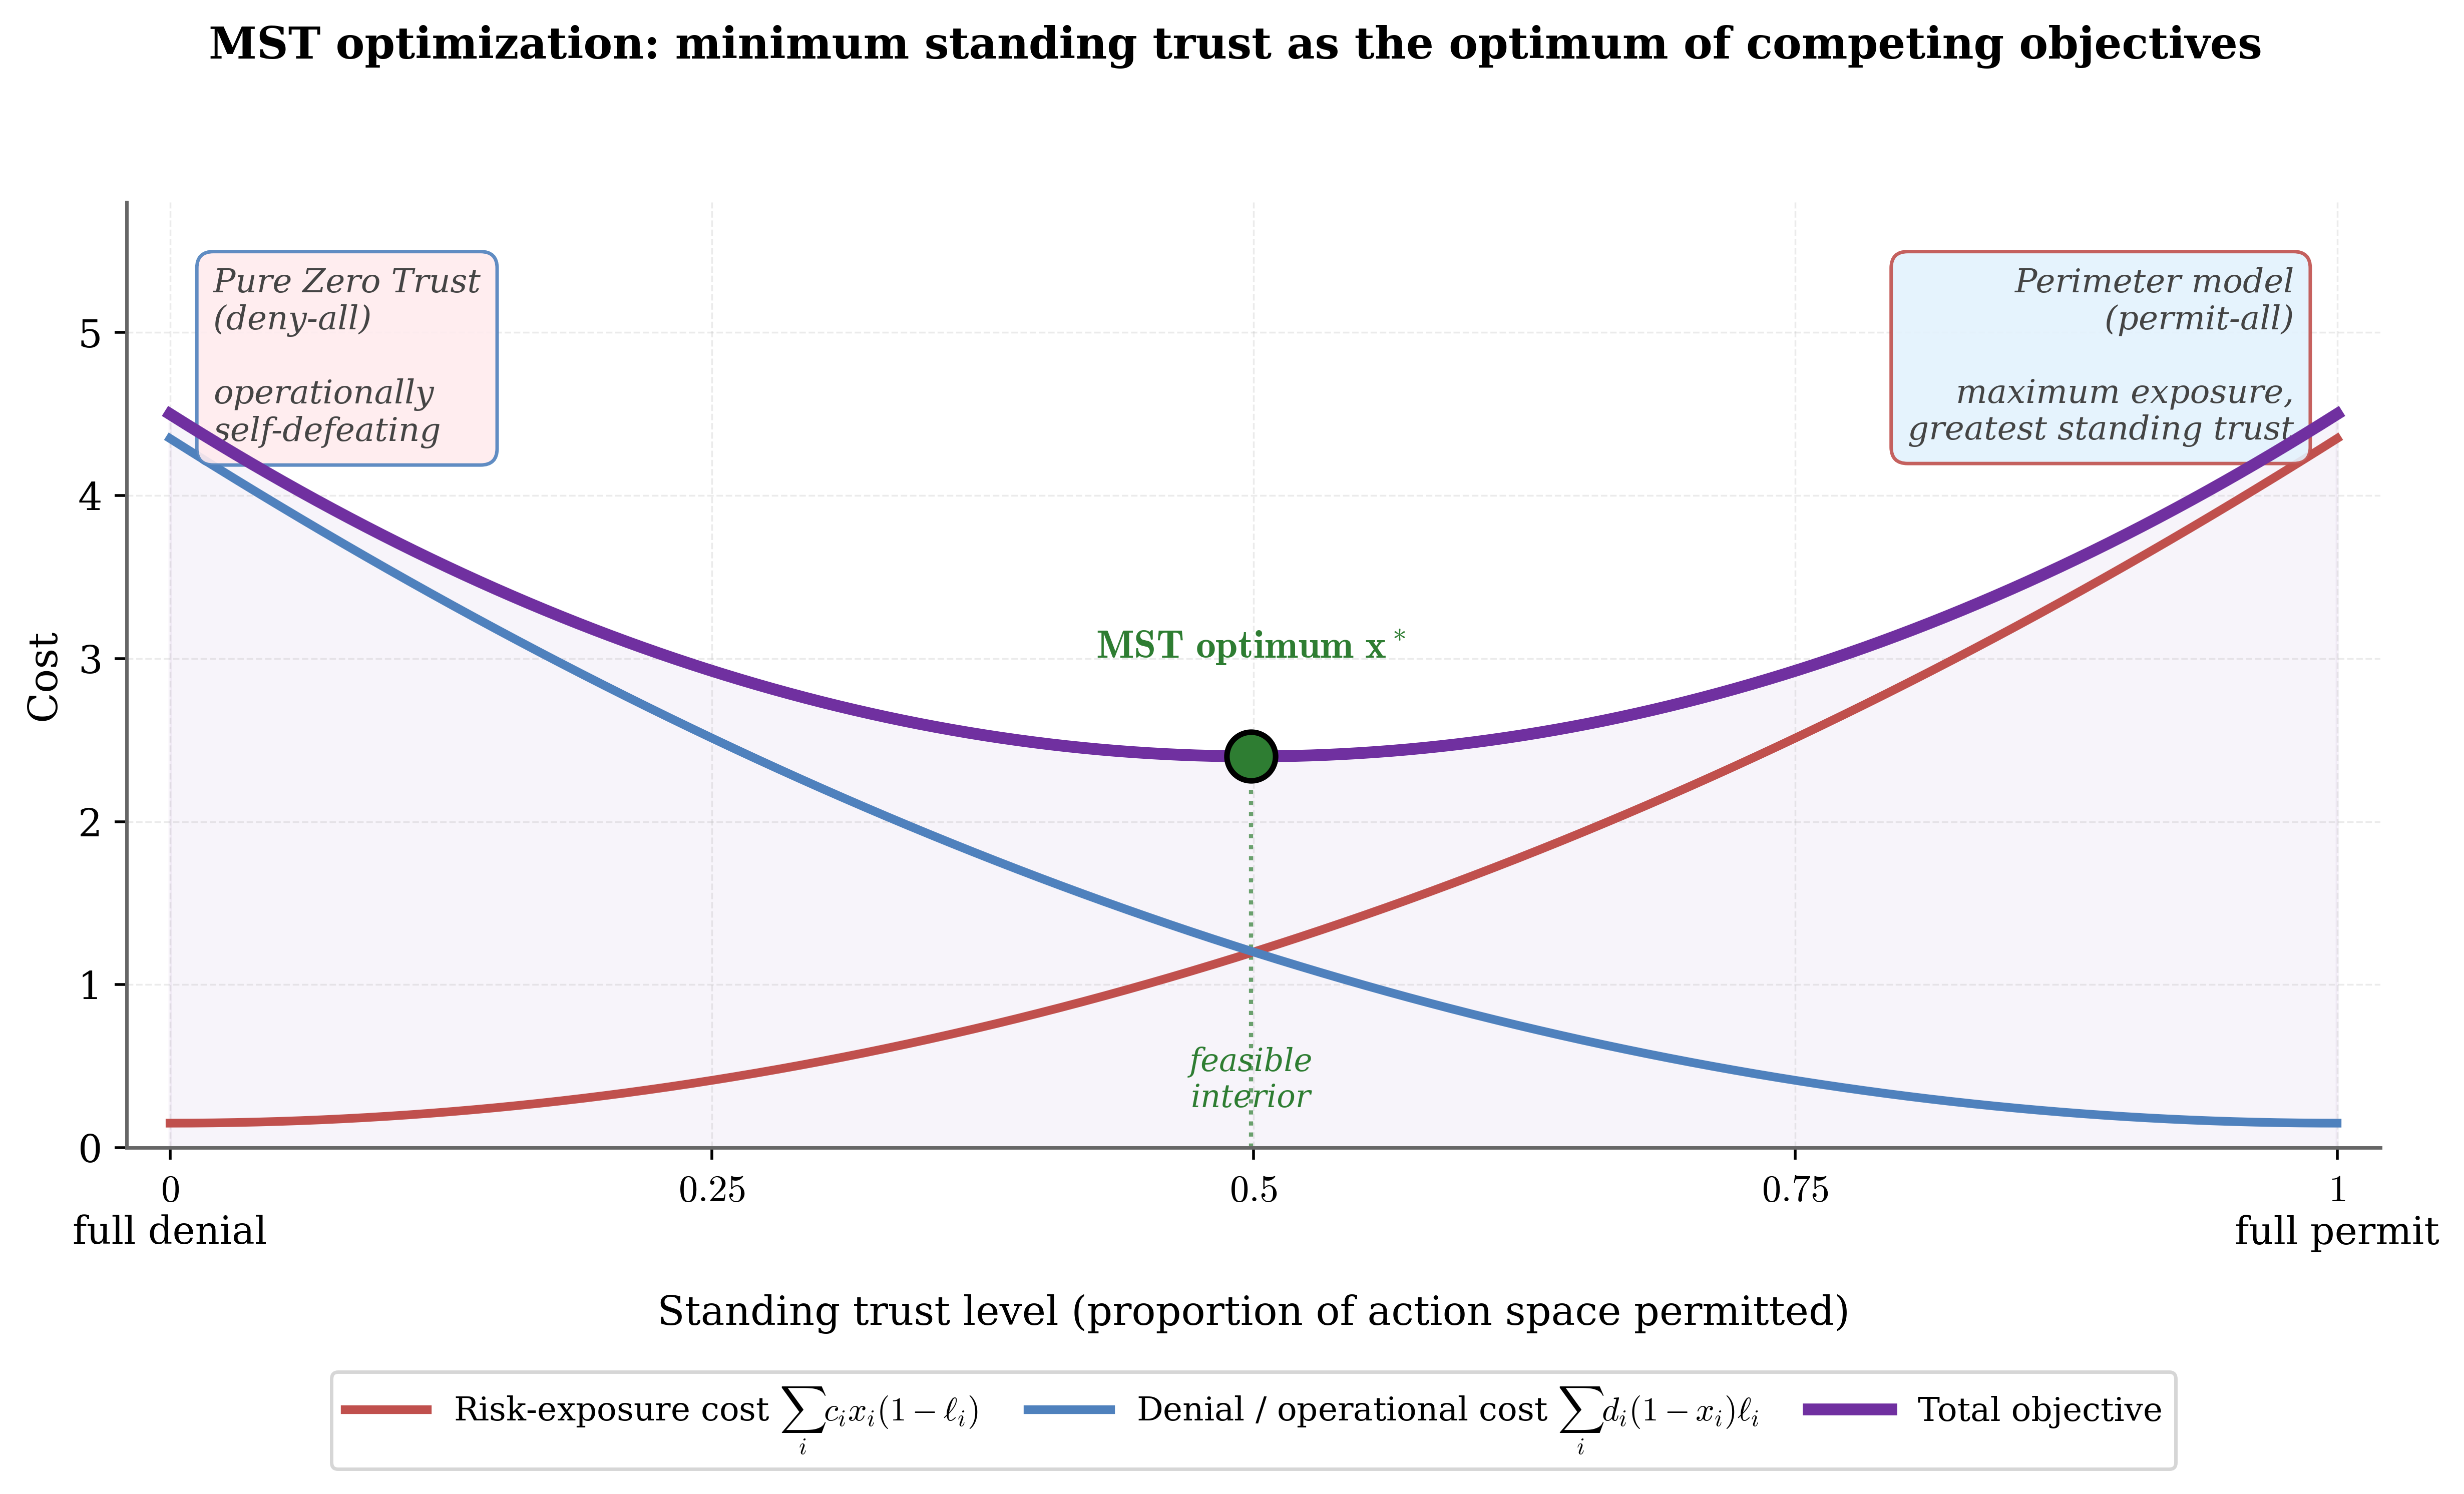
\includegraphics[width=0.92\textwidth]{figures/figure_mst_optimization_curve_500dpi.png}
\caption{The MST optimization geometry. The horizontal axis represents the
proportion of the action space that is permitted, ranging from full denial
($x_i=0\ \forall i$, left edge) to full permit ($x_i=1\ \forall i$, right edge).
The risk-exposure cost $\sum_i c_i\, x_i\, (1-\ell_i)$ is convex increasing in
permissiveness: more granted access exposes more attack surface. The denial /
operational cost $\sum_i d_i\, (1-x_i)\, \ell_i$ is convex decreasing: more
granted access denies fewer business-required actions. Their sum is the MST
total objective of Equation~(\ref{eq:mvt_weighted}), which is U-shaped on this
axis and attains its minimum at the feasible interior point $\mathbf{x}^*$:
the operating point of \textit{minimum standing trust consistent with
business-required operations}. Pure Zero Trust (deny-all) is operationally
self-defeating in this geometry; the perimeter model (permit-all) maximizes
exposure. The MST framework rejects both extremes and locates the optimum
between them.}
\label{fig:mst_optimization}
\end{figure*}

Figure~\ref{fig:mst_optimization} visualises this geometry. The U-shape of
the total objective is the central reason that adding controls monotonically
does not yield monotonic security improvement: past the MST optimum
$\mathbf{x}^*$, additional denial increases denial cost faster than it
reduces residual risk, and the security program absorbs operational damage
without commensurate benefit. Conversely, every unit of standing trust
granted to the right of $\mathbf{x}^*$ adds risk cost faster than it removes
operational friction. Identifying $\mathbf{x}^*$---and operating at it---is
therefore not merely a matter of policy preference but the explicit goal of
the MST framework.

\textbf{Limitations of the formulation.}
Several limitations of Equation~(\ref{eq:mvt_weighted}) deserve explicit
acknowledgement.

\textit{Action independence.} The formulation treats each action $a_i$ as
independent: the cost of permitting or denying $a_i$ does not depend on which other
actions are simultaneously permitted. In practice, actions are not independent.
Permitting a read on a regulated dataset and permitting an export to an external
endpoint together create an exfiltration path that neither action creates alone.
The independent-action assumption is the most consequential modelling simplification
in the formulation, and extending the model to capture combinatorial action
interactions---at the cost of substantially increased complexity---is an important
direction for future work.

\textit{Uniform action weight.} Each action is assigned a single scalar $c_i$,
treating all consequences of incorrectly permitting it as commensurable. In
practice, an action can have multiple consequence dimensions (regulatory, financial,
reputational, operational) that may not reduce to a single number without arbitrary
weighting choices. The $c_i$ parameterisation is therefore an abstraction that
organisations must calibrate carefully, and different calibrations will produce
materially different optimal policies.

\textit{The proxy hypothesis.} Equation~(\ref{eq:mvt_weighted}) optimises a
measurable cost function as a proxy for unmeasurable quantities such as
$P(\text{breach})$ or expected breach impact. The hypothesis that minimising
the weighted trust surplus reduces actual breach probability is operationally
motivated but not proven. It is the foundational modelling assumption of the MST
framework, not a derived result, and its empirical validation is identified in
Section~10 as a priority research direction.

\textit{Static $\mathcal{L}$.} The legitimate business-required set $\mathcal{L}$
is treated as known and fixed within each optimisation instance. In practice,
$\mathcal{L}$ is dynamic, incompletely specified, and contested: engineering teams
add new access requirements faster than governance processes can document them, and
emergency exceptions create persistent paths that were never formally added to
$\mathcal{L}$. The action-space-time graph formulation in Section~\ref{sec:theory_graph} partially
addresses this by indexing $\mathcal{L}^{(t)}$ over time, but it does not resolve
the harder problem of learning $\mathcal{L}$ from operational behaviour rather than
from policy declarations.



\subsection{Action-Space-Time Graph Formulation}
\label{sec:theory_graph}

The weighted ILP formulation of Equations~(\ref{eq:mvt_weighted})--(\ref{eq:c3}) treats the action space as a static flat set.
In practice, enterprise access patterns are dynamic: identities, devices, sessions,
and resources change state continuously, and the verification score $V(a_i, t)$ and
threshold $\theta(\rho_i, t)$ are time-varying quantities. A graph-theoretic
formulation captures this temporal dimension naturally.

Define the \textbf{action-space-time graph} $G = (V_G, E_G)$ as follows. The vertex
set $V_G = \mathcal{U} \cup \mathcal{R}$ partitions into \textit{actor nodes}
$\mathcal{U}$ (users, service accounts, processes, devices) and \textit{resource
nodes} $\mathcal{R}$ (data stores, APIs, administrative consoles, cloud control plane
endpoints). Each directed edge $e_{ij} \in E_G$ from actor node $u_i \in \mathcal{U}$
to resource node $r_j \in \mathcal{R}$ represents a potential access action, with
weight $c_{ij}$ encoding risk exposure. Time-indexed copies of the graph,
$G^{(t)} = (V_G, E_G^{(t)})$, capture the fact that verification scores and
business requirements evolve: an edge $e_{ij}$ that is permitted at time $t$ may
not satisfy the verification threshold at time $t + \Delta t$ if device posture
degrades or session context changes.

The MST problem on the graph is: find the minimum-cost subgraph
$G^* = (V_G, E^*)$ of $G^{(t)}$ such that:
\begin{enumerate}
  \item $E^*$ contains all edges corresponding to $\mathcal{L}^{(t)}$ (the
        current legitimate business-required actions);
  \item For every edge $e_{ij} \in E^*$: $V(e_{ij}, t) \geq \theta(r_j, t)$;
  \item The induced subgraph on $\mathcal{L}^{(t)}$ is connected in the sense
        that all business workflows can execute without interruption.
\end{enumerate}

The objective function on the graph is $\min_{E^*} \sum_{e_{ij} \in E^* \setminus
\mathcal{L}^{(t)}} c_{ij}$, i.e., minimize the total risk-exposure weight of
permitted edges that are not legitimately required. This is a \textit{weighted
minimum subgraph cover} problem on a bipartite directed graph. When $c_{ij} = 1$
for all edges, it reduces to the uniform cardinality formulation in
Equation~(\ref{eq:mvt}).

\begin{figure*}[h]
\centering
\includegraphics[width=\textwidth]{figureA1_subgraph_cover_500dpi.png}
\caption[]{\textbf{Weighted minimum subgraph cover: full action space $G$ and
optimal permitted subgraph $G^*$.} The left panel shows the full bipartite graph
of candidate access actions between three actor nodes ($\mathcal{U}$) and three
resource nodes ($\mathcal{R}$), with each directed edge labelled by its risk-exposure
weight $c_{ij}$ and current verification score $V$. The right panel shows the
MST-optimal permitted subgraph $G^*$: green edges are business-required and
pass the verification threshold; the amber dashed edge (U2$\to$R1) is not required
but has low $c=1$ cost so is retained; red dashed edges fail the verification
gate ($V < \theta$) and are ineligible regardless of business requirement. The
key illustrative case is U2$\to$R3: the Engineer needs control-plane access
($\ell=1$) but achieves only $V=0.79$, which falls below the critical-resource
threshold $\theta=0.95$. The policy response is not to lower $\theta$ but to
remediate the evidence gap---step-up authentication or device re-enrolment---before
the permission can be granted.}
\label{fig:subgraph}
\end{figure*}

This graph representation connects directly to intrusion detection systems that model
enterprise activity as a provenance graph or process-lineage graph
\cite{hassan2020provenance}. In those systems, nodes represent processes, files, and
network sockets, and edges represent system-call-level events---precisely the fine
granularity of the action space described here. The MST subgraph cover problem can
therefore be instantiated on a provenance graph, treating each system-level event as
a candidate $x_i$ and applying the verification and risk constraints per edge.
This connection makes the MST formulation amenable to empirical validation on
provenance graph datasets, a direction identified as a priority in Section~10.

\subsection{Complexity and Tractability}
\label{sec:theory_complexity}

The uniform-cardinality version of the MST problem (minimize $|\mathcal{T} \setminus
\mathcal{L}|$ subject to $\mathcal{L} \subseteq \mathcal{T}$ and verification
constraints) is equivalent, when the verification constraint is dropped, to
finding the minimum superset of $\mathcal{L}$ in $\mathcal{S}$, which is trivially
solvable. The computational difficulty arises from two sources: (1) the
verification constraint $V(a_i) \geq \theta(\rho_i)$ couples the permission
variables $x_i$ to a scoring function that may be non-linear and resource-intensive
to evaluate; (2) in the weighted formulation, the interaction between the two
objective terms and the completeness constraint creates a structure analogous to the
\textbf{0-1 knapsack problem}, which is NP-hard in the strong sense
\cite{garey1979}: each action $a_i$ has a ``profit'' (denial cost $d_i$ if it is
in $\mathcal{L}$) and a ``weight'' (risk cost $c_i$), and the problem is to select
the minimum-risk superset of $\mathcal{L}$ within the feasible verification region.

More precisely, the weighted MST problem (Equations~\ref{eq:mvt_weighted}--\ref{eq:c3})
is NP-hard by reduction from 0-1 knapsack: given a knapsack instance with items
$\{1,\ldots,n\}$, values $v_i$, weights $w_i$, and capacity $W$, construct an MST
instance with $\mathcal{L} = \emptyset$, $c_i = w_i$, $d_i = v_i$, and
$\theta(\rho_i) = 0$ for all $i$. The MST optimal selects the minimum-weight
feasible set, which corresponds directly to the knapsack optimal selection.

For practical enterprise scales, this complexity motivates relaxation approaches.
A \textbf{linear programming (LP) relaxation} of Equations~(\ref{eq:mvt_weighted})--(%
\ref{eq:c3}) replaces $x_i \in \{0,1\}$ with $x_i \in [0,1]$ and solves the
resulting LP in polynomial time; the fractional solution can be rounded to a
feasible integer solution with a bounded approximation ratio. Alternatively, the
structure of the problem---bipartite graph, separable objective, binary variables---
makes it well-suited to \textbf{branch-and-bound mixed integer programming (MIP)}
solvers, which handle enterprise-scale instances (tens of thousands of action
types) routinely in practice \cite{wolsey1998}. For real-time enforcement decisions,
where the full MIP is too slow, a greedy policy that sorts candidate actions by
$c_i / V(a_i, t)$ (risk per unit of verification evidence) and admits actions in
ascending risk order until the completeness constraint is satisfied provides a
practical approximation with a well-understood performance bound.

The time-varying graph formulation introduces additional structure: as $\theta(r_j, t)$
and $V(e_{ij}, t)$ change, previously permitted edges may need to be revoked and
previously denied edges may become admissible. The dynamic version of the problem
is related to \textit{online subgraph maintenance} under changing constraints, a
problem studied in the streaming graph algorithms literature
\cite{mcgregor2014streaming}. This connection suggests that the SOC's continuous
re-evaluation of session trust is not merely a policy preference but a computational
necessity: the optimal permitted set changes as the verification evidence changes,
and maintaining it requires incremental update rather than full re-solve.

\subsection{Mapping Optimization Elements to Architecture}
\label{sec:theory_mapping}

The formalization above maps directly onto the two-plane operating architecture and
unified telemetry framework described in Sections~4--7, as summarized below.

\textbf{Action space $\mathcal{S}$.} At the external application edge, the action
space is narrow: inbound HTTP/S requests, API calls, authentication attempts, and
partner integrations. The cardinality of $\mathcal{L}$ at the edge is small and
well-documented, making the optimization tractable and the verification threshold
$\theta$ enforceable close to deny-by-default. Internally, $|\mathcal{S}|$ is
orders of magnitude larger (every user-to-resource path across the enterprise),
but the risk weights $c_i$ concentrate on a small subset of high-consequence actions
(privileged administrative sessions, regulated data access, cloud control plane
operations), allowing the optimizer to allocate verification resources
proportionally.

\textbf{Verification score $V(a_i, t)$.} The unified telemetry plane (Section~7)
exists precisely to compute $V(a_i, t)$ in real time. Each source---IAM, EDR,
ZTNA, NIDS, UEBA---contributes a component of the verification score. Without
telemetry fusion, $V(a_i, t)$ cannot be computed accurately, and the optimization
problem becomes infeasible: actions are permitted or denied on incomplete evidence,
which corresponds to setting some $c_i$ to zero (under-penalizing risky actions)
or some $d_i$ to zero (under-protecting legitimate ones).

\textbf{Bounded autonomy as a constraint on $c_i$.} The bounded-autonomy ladder
(Section~8) is a policy translation of the risk-weight structure. Actions at the
top of the ladder (policy rewrites, permanent access changes) have high $c_i$ and
are therefore excluded from autonomous execution even when $V(a_i, t) \geq \theta$.
Actions at the bottom (alert enrichment, duplicate suppression) have negligible
$c_i$ and are freely automated. The ladder makes the optimization structure
operationally legible to analysts who do not interact with the formal model directly.

\textbf{Discussion of assumptions.} The MST model rests on the working hypothesis
that minimizing the risk-weighted unnecessary trust set $\sum_i c_i x_i (1 - \ell_i)$
is a useful proxy for minimizing concrete security metrics such as $P(\text{breach})$
or expected breach impact. This hypothesis is not proven in the paper; it is the
fundamental modeling assumption, analogous to the assumption in network hardening
that minimizing attack graph reach reduces breach probability \cite{shandilya2014}.
The advantage of the set-size and graph-size formulations is that they are
computable from operational data, whereas $P(\text{breach})$ is not. We acknowledge
this approximation and identify its empirical validation as a priority research
direction (Section~10).



\subsection{Attack Surface Minimization as the Theoretical Objective}
\label{sec:theory_surface}

The formulation of Equations~(\ref{eq:mvt})--(\ref{eq:c3}) has a direct interpretation
in the attack-surface-minimization literature introduced by work on attack surface metrics \cite{howard2005,manadhata2011}. In that
tradition, the \textit{attack surface} of a system is the subset of its resources
reachable and usable by an attacker: entry points through which inputs flow, exit points
through which outputs flow, and channel resources that mediate communication. Reducing
this surface reduces the opportunities available for adversarial exploitation.

For the MST framework, the connection is immediate. The permitted action set
$\mathcal{T} \subseteq \mathcal{S}$ \emph{is} the enterprise attack surface in the
relevant sense: every action permitted by policy is an action an attacker might
exploit if they can impersonate a legitimate actor or compromise the verification
context. The legitimate business-required set $\mathcal{L} \subseteq \mathcal{T}$ is
the irreducible lower bound on this surface---the portion that must be exposed for
the service to function---and the trust surplus $\mathcal{T} \setminus \mathcal{L}$
is the avoidable portion. The MST objective is therefore a direct quantitative
expression of attack surface minimization under operational feasibility constraints.

\textbf{The effect of reputation-based blocking.} A reputation-list control---whether
operated at the network perimeter (NIDS, firewall) or at the endpoint (EDR egress
policy)---modifies the problem structure by pre-filtering the action space itself,
not merely the permitted subset. Let $\mathcal{B} \subseteq \mathcal{S}$ denote the
set of actions whose identity tuple $a_i = (\iota_i, \delta_i, \rho_i, \sigma_i,
\omega_i)$ has either $\iota_i$ or $\rho_i$ resolving to an IP address on a curated
reputation feed. Reputation-based auto-blocking enforces $x_i = 0$ for every
$a_i \in \mathcal{B}$ regardless of all other considerations. The effective action
space becomes:
\begin{equation}
\mathcal{S}_{\text{eff}} = \mathcal{S} \setminus \mathcal{B}
\label{eq:s_effective}
\end{equation}
and the MST optimization is solved over $\mathcal{S}_{\text{eff}}$ rather than
$\mathcal{S}$. Because reputation feeds explicitly enumerate hosts with documented
adversarial activity, the expected intersection
$\mathcal{L} \cap \mathcal{B}$ is close to empty---legitimate business counterparties
do not appear on Spamhaus DROP or AbuseIPDB---so the completeness constraint
$\mathcal{L} \subseteq \mathcal{T}^{*}$ remains satisfiable in $\mathcal{S}_{\text{eff}}$.
The practical result is that the optimal permitted set $\mathcal{T}^{*}_{\text{eff}}$
computed over $\mathcal{S}_{\text{eff}}$ has strictly smaller attacker-exploitable
surface than the corresponding optimum $\mathcal{T}^{*}$ computed over the full
$\mathcal{S}$:
\begin{equation}
\bigl|\mathcal{T}^{*}_{\text{eff}} \setminus \mathcal{L}\bigr|
\;\leq\;
\bigl|\mathcal{T}^{*} \setminus \mathcal{L}\bigr|
\label{eq:surface_reduction}
\end{equation}
with strict inequality whenever $\mathcal{B}$ contains any action that would otherwise
satisfy the verification threshold under $\mathcal{T}^{*}$.

\textbf{The theoretical lower bound.} Equation~(\ref{eq:surface_reduction}) frames
the fundamental question of how far attack surface can be reduced in principle. The
global lower bound is given by the legitimate set itself:
\begin{equation}
\bigl|\mathcal{T}^{*} \setminus \mathcal{L}\bigr| \;\geq\; 0
\label{eq:global_bound}
\end{equation}
with equality if and only if every action in $\mathcal{T}^{*}$ is business-required.
This bound is achievable only under perfect information---complete knowledge of
$\mathcal{L}$, perfect verification ($V(a_i) = 1$ for all legitimate actions), and
no external dependencies. In practice, the realized trust surplus is strictly
positive, and the engineering question becomes: how close to zero can it be driven
without violating the operational-cost constraint?

The two planes of the MST architecture give different answers to this question.
At the external application edge, $\mathcal{L}$ is narrow, well-documented, and
relatively static (customer API calls, authentication endpoints, partner integrations),
making the trust surplus easier to drive toward zero. Bidirectional reputation
blocking reduces it further by shrinking the action space before the optimization
is even formulated. Inside the internal enterprise, $\mathcal{L}$ is broader,
dynamic, and incompletely specified, so the achievable minimum is inherently
larger---but endpoint-enforced reputation blocking still reduces it by an amount
bounded by the size of $\mathcal{B}$ restricted to internal-origin traffic.

The MST model thus provides both an operational framework and a theoretical
minimum: the ideal end-state of a Zero Trust program is a permitted action set
exactly equal to the current legitimate business-required set, with all other
actions either denied by policy or pre-filtered by reputation-based blocking.
Every deviation from this ideal---every permitted action outside $\mathcal{L}$,
every connection to or from a reputation-listed IP that the platform fails to
block---is a quantifiable gap in the architecture rather than an unmeasurable
policy judgement. This quantifiability is what distinguishes attack surface
minimization from traditional Zero Trust rhetoric: it supplies a target that
organizations can measure progress against, and it supplies a theoretical
justification for specific controls (reputation blocking, JIT privilege,
device tiering) in terms of the surface-reduction they produce.

%%% -----------------------------------------------------------------------
\section{Expected Outcomes and Argument Summary}
\label{sec:outcomes}

\subsection{Summary of the Central Argument}

The argument of this paper can be stated plainly. Zero Trust is not a product category.
Network location is not a trust signal. Standing privilege is the enemy. Compliance
evidence is a byproduct of good architecture, not its purpose. These are not marketing
slogans; they are operational commitments with specific engineering consequences.

The Minimum Standing Trust model operationalizes these commitments in four steps.
Step one: at the Internet-facing application edge, enforce deny-by-default using WAF,
NIDS, and abuse-list controls as \textit{instruments} of that posture---not as the
posture itself. Step two: inside the enterprise, eliminate standing privilege through
identity-centric access, device-trust tiering, JIT elevation, and continuous session
verification. The goal is that no adversary who acquires a credential can inherit the
access it once carried indefinitely. Step three: fuse all telemetry into a single
decision plane so that the security operations center receives incidents, not
fragments, and can answer who acted, from where, against what, with what evidence.
Step four: let AI operate inside this model---automating what is reversible, narrow,
and pre-authorized while requiring human judgment for anything that cannot be quickly
undone or that touches regulated data at scale. The compliance records that regulators
and auditors need are a natural output of this architecture, not a parallel
documentation effort.

\subsection{Expected Operational Outcomes}

A Zero Trust operations model is credible only if it produces measurable improvements
in outcomes rather than merely increasing control count or coverage claims. For a regulated
SaaS enterprise, the MST framework is expected to produce four principal outcome improvements.

\textbf{Reduction in unjustified access.} The progressive removal of standing trust,
JIT privilege, and device-trust tiering collectively shrink the attack surface available
to an adversary who has acquired a valid credential. This directly reduces the dwell time
and lateral movement capability implied by a credential-theft event. Credential and
identity-based attacks remain the dominant initial-access vector across all major annual
threat intelligence reports \cite{verizon2025,crowdstrike2025,ciscotalos2025}.

\textbf{Reduction in analyst toil.} Unified telemetry and bounded AI automation reduce
the manual correlation work imposed on analysts by fragmented detection stacks. Alert
enrichment, case summarization, and duplicate suppression are the highest-volume, lowest-value
analyst tasks; automating them within the bounded-autonomy framework frees analyst capacity
for high-judgment work such as threat hunting, policy refinement, and incident command.

\textbf{Improvement in detection and containment speed.} A shared telemetry pipeline with
pre-enriched incident records reduces mean-time-to-detect and mean-time-to-contain by
eliminating manual pivot time. When an analyst receives an incident rather than a fragment,
the time from alert to containment decision is reduced by the elimination of the context-assembly
phase.

\textbf{Improvement in audit-evidence generation.} Unified telemetry with compliance-tagged
event records transforms audit preparation from a retrospective evidence-gathering exercise
into a continuous operational byproduct. The evidence a regulator or customer questionnaire
requires---access logs, control outcomes, exception records, policy decisions---exists as a
natural output of the operational platform rather than a separately constructed artifact.

\subsection{Performance Metrics and Governance Cadence}

The appropriate scorecard for the MST framework balances four dimensions: security
effectiveness, analyst efficiency, business friction, and evidence quality. Useful
quantitative measures include: mean time to detect (MTTD); mean time to contain (MTTC);
mean time to recover (MTTR); false-block rate (the fraction of automated blocks that
are later reversed as erroneous); exception-turnaround time (time from exception request
to documented resolution); percentage of analyst time on repeatable low-value tasks;
percentage of autonomous actions subsequently reversed; and the fraction of alert volume
arriving with sufficient context to support a decision without manual pivoting.

In regulated environments, a further class of metrics is operationally essential: evidence
latency (how quickly can an event be reconstructed for audit?); control-to-case
traceability (can every control action be linked to a governing policy and a ticket?);
and answer time for auditor or customer inquiries about specific access events.

An explicit multi-objective optimization model is useful for framing governance reviews
honestly. Security teams are often informally evaluated on whether they block enough
adversarial activity while formally measured on availability, audit readiness, and
customer trust. These objectives can pull in opposite directions, and the temptation is
to resolve the tension implicitly rather than explicitly. The MST optimization structure (Section~\ref{sec:theory_action}, Equation~\ref{eq:mvt}) makes the tradeoff visible: reducing $|\mathcal{T} \setminus \mathcal{L}|$
is the security objective; maintaining $\mathcal{L} \subseteq \mathcal{T}$ is the
availability constraint; and the verification threshold $\theta$ parameterizes the
risk tolerance of the organization at each resource class. Governance reviews should
track all three dimensions simultaneously.

\subsection{Validation and Red-Team Considerations}

Validation must be explicit and structured. Edge policies should be exercised through
red-team and purple-team scenarios simulating exploit traffic, abuse-list hits,
false-attribution cases, and partner-traffic exceptions. Internal Zero Trust controls
should be tested against stolen-session scenarios, unmanaged-device access attempts,
privilege escalation paths, support-account misuse, and insider-style behavioral anomalies.
AI-enabled playbooks should be run in shadow mode with before-and-after comparison of
analyst actions, response speed, reversal rates, and business impact, before being
promoted to live execution authority.

Without structured validation, organizations tend to overestimate both detection precision
and readiness for autonomous action. The bounded-autonomy ladder in Figure~\ref{fig:autonomy_ladder}
and the decision matrix in Table~\ref{tab:decision_matrix} are useful not just as design
guides but as evaluation rubrics: an organization can assess whether its current autonomous
action program stays within the cells that the framework designates as safe for automation.

These reviews should engage more than the SOC. In a regulated SaaS company, the consequences
of Zero Trust policy are distributed across engineering, support, privacy, compliance,
product, and customer trust functions. A regular cross-functional governance cadence is
therefore essential. At minimum, the organization should review: the precision of automated
blocks; the exception patterns introduced by geo or reputation controls; the policy drift
introduced by repeated emergency overrides; the failure modes of behavioral detections; and
the cases in which bounded automation either prevented harm or created avoidable friction.
These reviews convert isolated lessons learned into structured policy refinement.

\subsection{Limitations and Scope Boundaries}

The MST framework addresses operational architecture and governance structure; it does not
prescribe specific tool vendors, identity provider configurations, or regulatory compliance
mappings. Organizations will need to adapt the framework's principles to their specific
regulatory context (HIPAA, PCI-DSS, GDPR, SOC 2, and others impose different specific
requirements), technology stack, workforce scale, and risk tolerance. The formal model in
Section~\ref{sec:theory_action} is intended to clarify the optimization structure rather than to be computed
algorithmically in practice; the $V(a)$ scoring function and the $\theta$ thresholds are
policy parameters that each organization must define based on its own risk profile and
data classification standards.

The framework also does not resolve the challenge of third-party and supply-chain trust.
SaaS providers depend on cloud infrastructure, open-source components, and vendor integrations
that introduce trust relationships outside the direct control of the enterprise security
program. While the two-plane architecture provides a structural basis for evaluating
third-party access, a full supply-chain Zero Trust model is a substantial research and
operational program in its own right, and is identified as a direction for future work.

\subsection{Synthesis of the Theoretical Framework}
\label{sec:outcomes_theory}

The formal development in Section~\ref{sec:theory} can be summarized in five
interlocking elements that together transform Zero Trust from a posture
into an explicit constrained-optimization program.

\textit{The objective function.} Equation~\ref{eq:mvt} expresses the MST
problem as the minimization of a two-term cost: the risk-exposure cost
$\sum_i c_i\, x_i\, (1-\ell_i)$ of permitted actions outside the
business-required set, plus the operational-friction cost
$\sum_i d_i\, (1-x_i)\, \ell_i$ of denied legitimate actions, subject to
business completeness, verification sufficiency
($V(a_i, t) \geq \theta(\rho_i, t)$), and binary integrality. The two
opposing terms make explicit the trade-off that Zero Trust programs
otherwise resolve implicitly and badly. The risk-exposure weights $c_i$,
the denial costs $d_i$, and the resource-sensitive thresholds
$\theta(\rho_i, t)$ are policy parameters that organizations calibrate to
their own data classification and operational tolerance; the framework
specifies their roles, not their values.

\textit{The decision variables.} The action tuple
$a_i = (\iota_i, \delta_i, \rho_i, \sigma_i, \omega_i)$ captures the
five dimensions an MST-aligned policy must consider for every access
decision: identity, device tier, resource and data classification,
session context, and requested operation. Treating these jointly---rather
than as independent gates---is what distinguishes MST from earlier
RBAC, ABAC, and policy-administrator-only formalizations.

\textit{The graph formulation.} The action-space-time graph
$G^{(t)} = (V_G, E_G^{(t)})$ casts the MST optimum as the
\textit{weighted minimum subgraph cover} of business-required edges
under time-varying verification weights. This formulation makes time
explicit, makes the connection to provenance-graph datasets concrete,
and provides a natural substrate for empirical evaluation.

\textit{The complexity result.} The weighted MST problem is NP-hard via
reduction from 0-1 knapsack. Tractable approaches---LP relaxation,
branch-and-bound MIP, greedy risk-ratio approximation, and online/streaming
formulation---make the model solvable in practice at enterprise scale,
and they explain why continuous re-evaluation of session trust in
operational SOCs is a computational requirement rather than merely a
policy preference.

\textit{The attack-surface implication.} The MST permitted action set
$\mathcal{T}^{*}$ \textit{is} the enterprise attack surface in the
established Manadhata--Wing sense. The MST objective is therefore a
direct quantitative expression of attack surface minimization under
operational feasibility constraints, with reputation-based pre-filtering
shrinking the effective action space $\mathcal{S}_{\text{eff}}$ before
optimization. Every gap between the realized $\mathcal{T}^{*}$ and the
business-required minimum $\mathcal{L}$ is a measurable architectural
deficit rather than an unmeasurable policy judgement.

\subsection{Future Work}
\label{sec:future_work}

Five research directions emerge directly from the framework.

\textit{Empirical validation of the proxy hypothesis.} The foundational
modelling assumption of MST---that minimising the risk-weighted trust
surplus is a reliable proxy for reducing breach probability or expected
breach impact---is operationally motivated but not proven. Longitudinal
study of Zero Trust maturity against observed security outcomes is the
primary research direction; the growing corpus of enterprise ZT
deployment data identified in the multivocal review~\cite{buck2021}
makes such study increasingly tractable.

\textit{Provenance-graph instantiation of the action-space-time graph.}
The MST subgraph cover formulation can be instantiated on public
provenance-graph datasets (e.g.\ those used in
OmegaLog~\cite{hassan2020provenance}), treating each system-call-level
event as a candidate $x_i$ and applying the verification and risk
constraints per edge. This would provide the first quantitative comparison
of MST-based access policy against baseline access-control regimes at
realistic granularity.

\textit{Action-independence extensions.} The current formulation treats
each action as independent. Extending the model to capture
combinatorial interactions---for instance, with pairwise risk terms
$c_{ij}\, x_i\, x_j$ for action pairs known to compose into higher-risk
compound actions (a read on regulated data plus an export to an external
endpoint, for example)---substantially increases computational complexity
but is essential for capturing real exfiltration paths. A principled
treatment of compound-action risk is an important next step.

\textit{Learning the legitimate set $\mathcal{L}$ from operational
behaviour.} Organizations maintain $\mathcal{L}$ through policy
declarations that lag operational reality. Time-indexed Bayesian updates,
semi-supervised clustering, or other behavioural-learning approaches
could close the gap between declared and effective legitimate sets, and
would integrate naturally with the UEBA evidence layer~\cite{tuor2017}
that already feeds the verification score $V(a_i, t)$.

\textit{Supply-chain extension.} The current two-plane architecture
addresses the enterprise's direct attack surface. SaaS providers depend
on cloud infrastructure, open-source components, and vendor integrations
that introduce trust relationships outside direct control. Extending MST
to fourth-party trust---where actions $a_i$ may be initiated by entities
whose identity and device tier are not directly observable to the
enterprise---is a substantial research program in its own right and a
natural next direction.

\section{Conclusion}
\label{sec:conclusion}

Zero Trust is not a product category. Network location is not a trust signal.
Standing privilege is the enemy. Compliance evidence is a byproduct of good
architecture, not its purpose.

These four commitments are not rhetorical. Each has a specific operational consequence.
Zero Trust is not a product category means that no tool purchase implements it;
it is a continuous operating discipline enacted through policy, verification, and
governance. Network location is not a trust signal means that being inside the
corporate network confers nothing; every access decision requires current evidence
of identity, device posture, and session legitimacy. Standing privilege is the enemy
means that persistent access grants---service accounts, never-expiring tokens,
broadly scoped admin roles---are the attack surface that adversaries actually
exploit, and eliminating them is the highest-leverage security investment an
organization can make. Compliance evidence is a byproduct means that organizations
that build good architecture generate the audit records regulators need as a
side-effect; organizations that build for compliance and treat security as secondary
get neither.

In a regulated SaaS enterprise, the Minimum Standing Trust framework operationalizes
these commitments: deny-by-default at the exposed application edge; identity-,
device-, and session-aware internal control with JIT privilege throughout; unified
telemetry across detection and access systems; and policy-governed AI autonomous
response bounded by the same trust criteria that govern human access.

The MST framework presented in this paper makes four contributions to the Zero Trust
literature.

First, it reframes the Zero Trust implementation problem as a constrained optimization
with competing objectives---minimizing unnecessary trust while preserving operational
completeness---and shows why monotonic control accumulation fails as a strategy.
This reframing explains empirically documented implementation failures that prior
frameworks left without a structural account \cite{buck2021}.

Second, it prescribes asymmetric enforcement posture across the two planes and
sharpens the control hierarchy: WAF, NIDS, and reputation controls are edge
instruments, not strategy; identity, device posture, JIT privilege, and session
verification are the substance of Zero Trust in the internal enterprise.

Third, it establishes unified telemetry as a correctness requirement of the MST
model---not a convenience---and provides a four-stage pipeline architecture
(Decoder, Alerting, Enrichment, Enriched Incident) that operationalizes this
requirement at the decision layer rather than at the dashboard layer.

Fourth, it integrates AI governance into the MST model as a first-class concern,
showing that the same trust criteria governing human access decisions govern AI
autonomous response actions, and providing the bounded-autonomy ladder as a
practical policy instrument for both.

A consequence of these four contributions, developed formally in
Sections~\ref{sec:theory_failure}--\ref{sec:theory_mapping}, is that the MST optimum corresponds to a principled
minimum on the enterprise attack surface in the established attack-surface sense \cite{manadhata2011}: the permitted action set $\mathcal{T}^{*}$ is the smallest
attacker-exploitable surface consistent with the organization's business requirements.
Bidirectional reputation-based blocking, applied symmetrically at both the network
perimeter and the endpoint, further reduces the effective action space by removing
from consideration any action whose counterparty is already known to be adversarial.
The full mathematical formalization, including the weighted ILP, action-space-time
graph, complexity analysis, and solution approaches, appears in
Sections~\ref{sec:theory_failure}--\ref{sec:theory_mapping}.

This operating model does not solve every problem. It does, however, close the gap between
Zero Trust in theory and cyber defense in practice. It gives the vSOC a clearer decision
surface. It reduces the standing privilege that adversaries can inherit through credential
compromise. It creates a structured path for AI-assisted defense without surrendering policy
authority to opaque automation. And it generates the evidence a regulated SaaS provider
needs not only to defend its platform, but also to explain its controls to customers,
auditors, and regulators.

For organizations operating under the mobile, distributed, and data-regulated conditions
that now characterize modern enterprise computing, the MST framework offers a practical
and theoretically grounded path to the intersection of Zero Trust principles and effective
cyber defense operations.

\textbf{Future work.} Several important directions remain open. The most pressing empirical question is whether the MST model's core
hypothesis holds in practice: that eliminating standing trust---measured by
credential exposure, dwell time, and lateral movement reach---is a reliable
proxy for reducing breach impact.
Longitudinal studies of Zero Trust maturity and security outcomes,
building on the multivocal review methodology of Buck et al.\ \cite{buck2021},
would provide a rigorous empirical path to this validation.
Instantiating the action-space-time graph on provenance graph datasets
\cite{hassan2020provenance} would provide a concrete experimental substrate for
evaluating the MST subgraph cover formulation at system-call granularity.
Developing efficient MIP formulations calibrated to enterprise-scale action spaces---
leveraging the bipartite structure of the actor-resource graph to reduce problem
dimensionality---is a tractable near-term algorithmic research agenda. The
extension of the two-plane architecture to supply-chain and fourth-party trust
relationships introduces additional graph layers (vendor nodes, dependency edges)
whose MST formulation remains open. Finally, the governance implications of
agentic AI in security operations---including the formal treatment of
irreversibility constraints on the $x_i$ variables, liability for autonomous
access decisions, and regulatory standards for AI-governed policy enforcement---
are emerging questions at the intersection of computer science and law that the
security research community is well-positioned to address.





\section*{Conflicts of Interest}
All three authors are affiliated with Athena Security Group. Peter J. Worth Jr. is founder, president, and CEO of Athena Security Group, and is concurrently a PhD candidate in the Department of Electrical Engineering and Computer Science at Florida Atlantic University. Dr. Ionut Cardei is a Professor in the Department of Electrical Engineering and Computer Science at Florida Atlantic University and serves as Chief Scientist at Athena Security Group. Dr. Chase Cunningham serves on the Leadership team of Athena Security Group and is the founder of the Dr. Zero Trust podcast. Athena Core and Athena Pallas are discussed in the paper only as disclosed implementation examples of the unified telemetry and AI-assisted response patterns described by the Minimum Standing Trust framework; the framework is intended to be vendor-neutral and applicable beyond any specific product or platform.

\section*{Funding}
No external funding supported this manuscript.

\section*{Data Availability}
No datasets were generated or analyzed during the preparation of this conceptual and operational framework paper.

\begin{acks}
The authors thank colleagues at Florida Atlantic University's Department of Electrical Engineering and Computer Science and at Athena Security Group for discussions that informed this work.
\end{acks}


\bibliographystyle{ACM-Reference-Format}
\bibliography{reference}

\end{document}
